%definira klasu dokumenta 
\documentclass[12pt]{report} 

%prostor izmedu naredbi \documentclass i \begin{document} se zove uvod. U njemu se nalaze naredbe koje se odnose na cijeli dokument

%osnovni LaTex ne može riješiti sve probleme, pa se koriste različiti paketi koji olakšavaju izradu željenog dokumenta
\usepackage{babel} 
\usepackage{amssymb}
\usepackage{amsmath}
\usepackage{txfonts}
\usepackage{mathdots}
\usepackage{titlesec}
\usepackage{array}
\usepackage{lastpage}
\usepackage{etoolbox}
\usepackage{tabularray}
\usepackage{color, colortbl}
\usepackage{adjustbox}
\usepackage{geometry}
\usepackage[classicReIm]{kpfonts}
\usepackage{hyperref}
\usepackage{fancyhdr}
\usepackage{graphicx}

\usepackage{float}
\usepackage{setspace}
\restylefloat{table}


\patchcmd{\chapter}{\thispagestyle{plain}}{\thispagestyle{fancy}}{}{} %redefiniranje stila stranice u paketu fancyhdr

%oblik naslova poglavlja
\titleformat{\chapter}{\normalfont\huge\bfseries}{\thechapter.}{20pt}{\Huge}
\titlespacing{\chapter}{0pt}{0pt}{40pt}


\linespread{1.3} %razmak između redaka

\geometry{a4paper, left=1in, top=1in,}  %oblik stranice

\hypersetup{ colorlinks, citecolor=black, filecolor=black, linkcolor=black,	urlcolor=black }   %izgled poveznice


%prored smanjen između redaka u nabrajanjima i popisima
\newenvironment{packed_enum}{
	\begin{enumerate}
		\setlength{\itemsep}{0pt}
		\setlength{\parskip}{0pt}
		\setlength{\parsep}{0pt}
	}{\end{enumerate}}

\newenvironment{packed_item}{
	\begin{itemize}
		\setlength{\itemsep}{0pt}
		\setlength{\parskip}{0pt}
		\setlength{\parsep}{0pt}
	}{\end{itemize}}




%boja za privatni i udaljeni kljuc u tablicama
\definecolor{LightBlue}{rgb}{0.9,0.9,1}
\definecolor{LightGreen}{rgb}{0.9,1,0.9}

%Promjena teksta za dugačke tablice
\DefTblrTemplate{contfoot-text}{normal}{Nastavljeno na idućoj stranici}
\SetTblrTemplate{contfoot-text}{normal}
\DefTblrTemplate{conthead-text}{normal}{(Nastavljeno)}
\SetTblrTemplate{conthead-text}{normal}
\DefTblrTemplate{middlehead,lasthead}{normal}{Nastavljeno od prethodne stranice}
\SetTblrTemplate{middlehead,lasthead}{normal}

%podesavanje zaglavlja i podnožja

\pagestyle{fancy}
\lhead{Programsko inženjerstvo}
\rhead{WildTrack}
\lfoot{Zoolanders}
\cfoot{stranica \thepage/\pageref{LastPage}}
\rfoot{\today}
\renewcommand{\headrulewidth}{0.2pt}
\renewcommand{\footrulewidth}{0.2pt}


\begin{document} 
	
	
	
	\begin{titlepage}
		\begin{center}
			\vspace*{\stretch{1.0}} %u kombinaciji s ostalim \vspace naredbama definira razmak između redaka teksta
			\LARGE Programsko inženjerstvo\\
			\large Ak. god. 2023./2024.\\
			
			\vspace*{\stretch{3.0}}
			
			\huge WildTrack\\
			\Large Dokumentacija, Rev. \textit{1}\\
			
			\vspace*{\stretch{12.0}}
			\normalsize
			Grupa: \textit{Zoolanders}\\
			Voditelj: \textit{Filip Ljubotina}\\
			
			
			\vspace*{\stretch{1.0}}
			Datum predaje: \textit{17.11.2023.}\\
	
			\vspace*{\stretch{4.0}}
			
			Nastavnik: \textit{Hrvoje Nuić}\\
		
		\end{center}

	
	\end{titlepage}

	
	\tableofcontents


	\chapter{Dnevnik promjena dokumentacije}
		
		\textbf{\textit{Kontinuirano osvježavanje}}\\
				
		
		\begin{longtblr}[
				label=none
			]{
				width = \textwidth, 
				colspec={|X[2]|X[13]|X[3]|X[3]|}, 
				rowhead = 1
			}
			\hline
			\textbf{Rev.}	& \textbf{Opis promjene/dodatka} & \textbf{Autori} & \textbf{Datum}\\[3pt] \hline
			0.1 & Napravljen predložak.	& Filip Ljubotina & 29.10.2023. 		\\[3pt] \hline 
			0.2	& Dopisane upute za povijest dokumentacije.\newline Dodane reference. & * & 24.08.2013. 	\\[3pt] \hline 
			0.5 & Dodan \textit{Use Case} dijagram i jedan sekvencijski dijagram, funkcionalni i nefunkcionalni zahtjevi i dodatak A & * & 25.08.2013. \\[3pt] \hline 
			0.6 & Arhitektura i dizajn sustava, algoritmi i strukture podataka & * & 26.08.2013. \\[3pt] \hline 
			0.8 & Povijest rada i trenutni status implementacije,\newline Zaključci i plan daljnjeg rada & * & 28.08.2013. \\[3pt] \hline 
			0.9 & Opisi obrazaca uporabe & * & 07.09.2013. \\[3pt] \hline 
			0.10 & Preveden uvod & * & 08.09.2013. \\[3pt] \hline 
			0.11 & Sekvencijski dijagrami & * & 09.09.2013. \\[3pt] \hline 
			0.12.1 & Započeo dijagrame razreda & * & 10.09.2013. \\[3pt] \hline 
			0.12.2 & Nastavak dijagrama razreda & * & 11.09.2013. \\[3pt] \hline 
			\textbf{1.0} & Verzija samo s bitnim dijelovima za 1. ciklus & * & 11.09.2013. \\[3pt] \hline 
			1.1 & Uređivanje teksta -- funkcionalni i nefunkcionalni zahtjevi & * \newline * & 14.09.2013. \\[3pt] \hline 
			1.2 & Manje izmjene:Timer - Brojilo vremena & * & 15.09.2013. \\[3pt] \hline 
			1.3 & Popravljeni dijagrami obrazaca uporabe & * & 15.09.2013. \\[3pt] \hline 
			1.5 & Generalna revizija strukture dokumenta & * & 19.09.2013. \\[3pt] \hline 
			1.5.1 & Manja revizija (dijagram razmještaja) & * & 20.09.2013. \\[3pt] \hline 
			\textbf{2.0} & Konačni tekst predloška dokumentacije  & * & 28.09.2013. \\[3pt] \hline 
			&  &  & \\[3pt] \hline	
		\end{longtblr}
	
	
		\textit{Moraju postojati glavne revizije dokumenata 1.0 i 2.0 na kraju prvog i drugog ciklusa. Između tih revizija mogu postojati manje revizije već prema tome kako se dokument bude nadopunjavao. Očekuje se da nakon svake značajnije promjene (dodatka, izmjene, uklanjanja dijelova teksta i popratnih grafičkih sadržaja) dokumenta se to zabilježi kao revizija. Npr., revizije unutar prvog ciklusa će imati oznake 0.1, 0.2, …, 0.9, 0.10, 0.11.. sve do konačne revizije prvog ciklusa 1.0. U drugom ciklusu se nastavlja s revizijama 1.1, 1.2, itd.}
	\chapter{Opis projektnog zadatka}
		
		Cilj projekta jest razviti web aplikaciju za olakšavanje koordinacije i praćenja životinja u divljini. Aplikacija omogućuje korisnicima da se prijavljuju i time sudjeluju u različitim akcijama.
		
		Pri učitavanju web aplikacije, neregistriranom korisniku omogućena je prijava u sustav s postojećim računom (potrebno je upisati korisničko ime ili email adresu i lozinku) ili kreiranje računa. Za kreiranje novog računa potrebni su sljedeći podaci:
		\begin{packed_item}
			\item ime
			\item prezime
			\item fotografija
			\item email adresa
			\item korisničko ime
			\item lozinka
		\end{packed_item}
		
		\begin{figure}[H]
			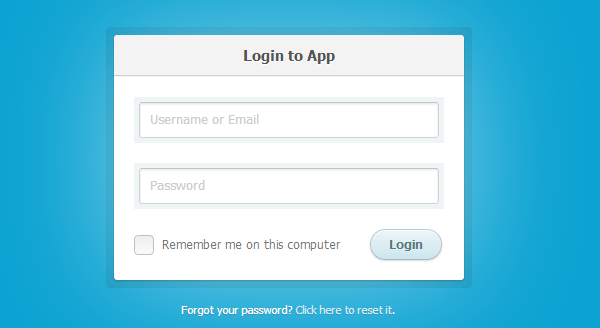
\includegraphics[scale=0.7]{slike/login_screen.PNG} %veličina slike u odnosu na originalnu datoteku i pozicija slike
			\centering
			\caption{Primjer login screena}
			\label{fig:promjene}
		\end{figure}
		
		%unos slike
		\begin{figure}[H]
			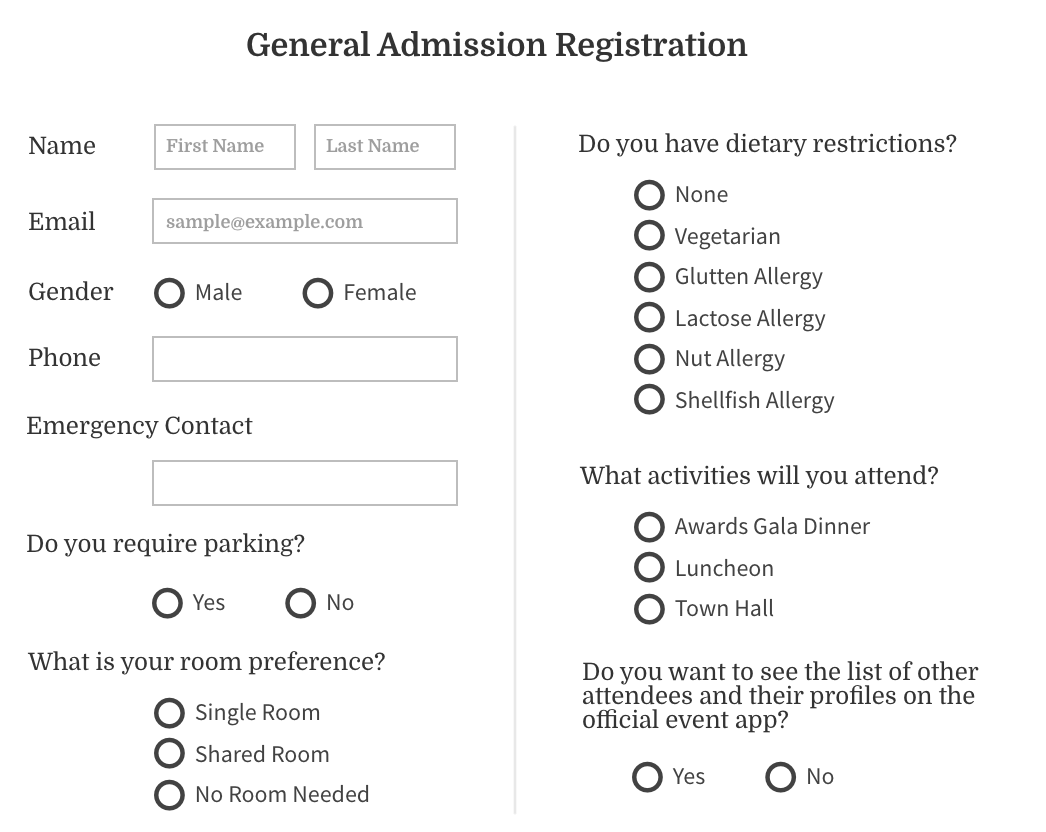
\includegraphics[scale=0.7]{slike/login_screen2.PNG} %veličina slike u odnosu na originalnu datoteku i pozicija slike
			\centering
			\caption{Primjer registracije}
			\label{fig:promjene}
		\end{figure}
		
		Pri registraciji korisnik također mora odabrati jednu od navedenih uloga:
		\begin{packed_item}
			\item voditelj postaje
			\item istražitelj
			\item tragač
		\end{packed_item}
		
		\begin{figure}[H]
			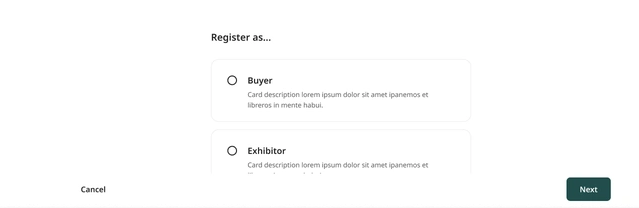
\includegraphics[scale=0.7]{slike/biranje_uloge.PNG} %veličina slike u odnosu na originalnu datoteku i pozicija slike
			\centering
			\caption{Primjer biranja uloge voditelja i unos željene postaje}
			\label{fig:promjene}
		\end{figure}
		
		U slučaju odabira uloge voditelja postaje, korisnik dodatno mora odabrati za koju postaju se želi registrirati.
		Registracija korisnika potvrđuje se mailom, a u slučaju registracije za ulogu \textit{istraživača} ili \textit{voditelja postaje} potrebna je i dodatna potvrda od strane administratora.
		Registrirani korisnik može pregledati svoje osobne podatke.
		
		\textbf{Voditelj postaje} ima pregled svih članova postaje. Omogućeno mu je dodavanje novih tragača u postaju i uklanjanje dosadašnjih. Voditelj postaje je ujedno zadužen i za definiranje na koji su način tragači osposobljeni izvoditi pretraživanje. Mogući načini izvođenja pretrage su:
		
		\begin{packed_item}
			\item pješke
			\item dronom
			\item automobilom
			\item cross motorom
			\item brodom
			\item helikopterom
		\end{packed_item}
		
		Svaka metoda pruža različitu vidljivost i područje pokrivanja. Na primjer, zračno pretraživanje će obuhvatiti veće područje, ali neće pružiti toliko detalja kao što bi se dobilo pješačenjem.
		
		Još jedna bitna zadaća voditelja postaje je da alocira svoje tragače prema pristiglim zahtjevima od strane istražitelja. Voditelj šalje tragača na sudjelovanje u navedenoj akciju, a smije ga maknuti s akcije i ponovno učiniti raspoloživim isključivo ako je tragač završio sa svojim zadatkom u toj akciji.
		
	\begin{figure}[H]
			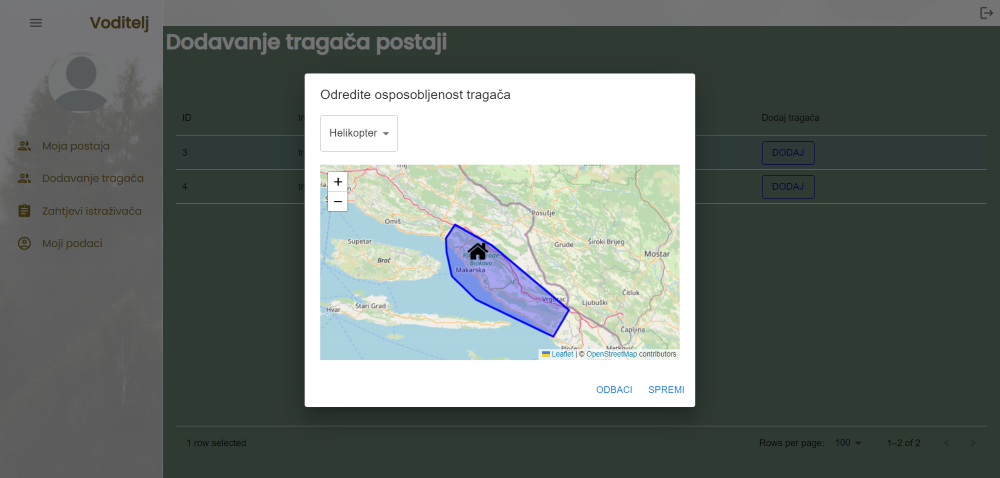
\includegraphics[scale=0.7]{slike/pr_biranja_osposobljenja.PNG} %veličina slike u odnosu na originalnu datoteku i pozicija slike
			\centering
			\caption{Primjer biranja osposobljenja tragača (1)}
			\label{fig:promjene}
		\end{figure}
		
		\begin{figure}[H]
			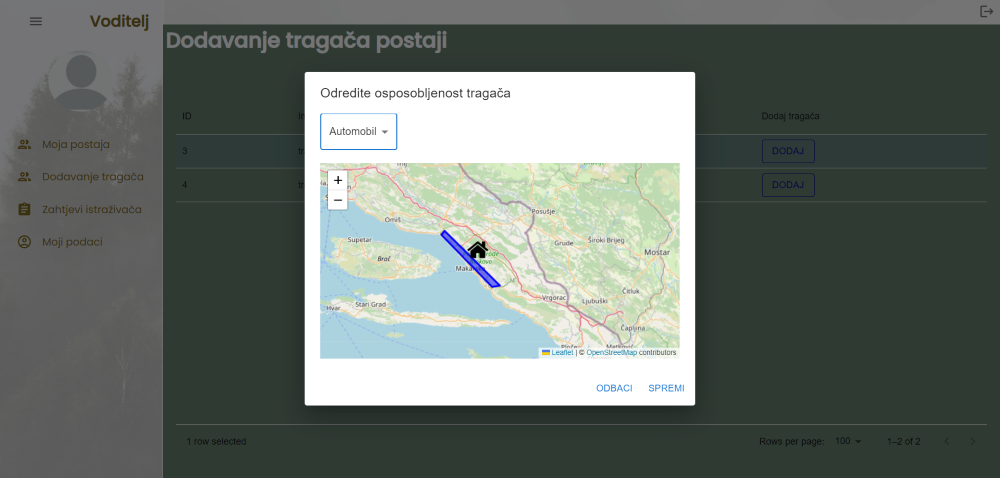
\includegraphics[scale=0.7]{slike/pr_biranja_osposobljenja2.PNG} %veličina slike u odnosu na originalnu datoteku i pozicija slike
			\centering
			\caption{Primjer biranja osposobljenja tragača (2)}
			\label{fig:promjene}
		\end{figure}
		
		\textbf{Istraživač} je osoba koja ne pripada niti jednoj postaji, a njegova uloga je organizacija akcija pretraživanja i praćenja s detaljima o određenim vrstama, jedinkama ili staništima za proučavanje. Istraživač može stvoriti novu akciju sa svim potrebnim detaljima te poslati zahtjeve za tragačima  s opisom o potrebnim kvalifikacijama voditeljima različitih postaje. On ima pregled svih akcija koje je pokrenuo, kao i tragača koji sudjeluju u tim akcijama. Istraživač preko karte tragačima pojedinačno zadaje zadatke. Definiran zadatak podrazumijeva prolazak tragača određenom rutom te postavljanje kamere ili uređaja za praćenje. Svaki zadatak može imati i dodatan komentar od istraživača. Istraživač je taj koji po završetku zadatka označava da je tragač s njim završio.
		
		Glavni alat dostupan istraživaču je interaktivna karta. Njome se istraživaču prikazuju informacije o pozicijama životinja, tragača i postaja, a istraživač može izabrati da se za njenu izradu koristi neka od idućih informacija: 
		
		\begin{packed_item}
			\item povijesne pozicije svih praćenih životinja, filtrirano po vrsti ili pojedinačno po jedinki 
			\item trenutne pozicije praćenih životinja
			\item povijesne pozicije svih tragača na nekoj akciji, filtrirano po tipu prijevoza ili pojedinačno po tragaču 
			\item trenutne pozicije tragača aktivnih na akciji
		\end{packed_item}
		
		Informacije o povijesnim pozicijama se prikazuju preko toplinskih karata (engl. heatmap). Toplinske karte prikazuju relativnu gustoću kretanja tragača i životinja određenim prostorom, a služe kako bi istraživač mogao analizirati obrasce kretanja životinja i omiljena staništa.
		
		\begin{figure}[H]
			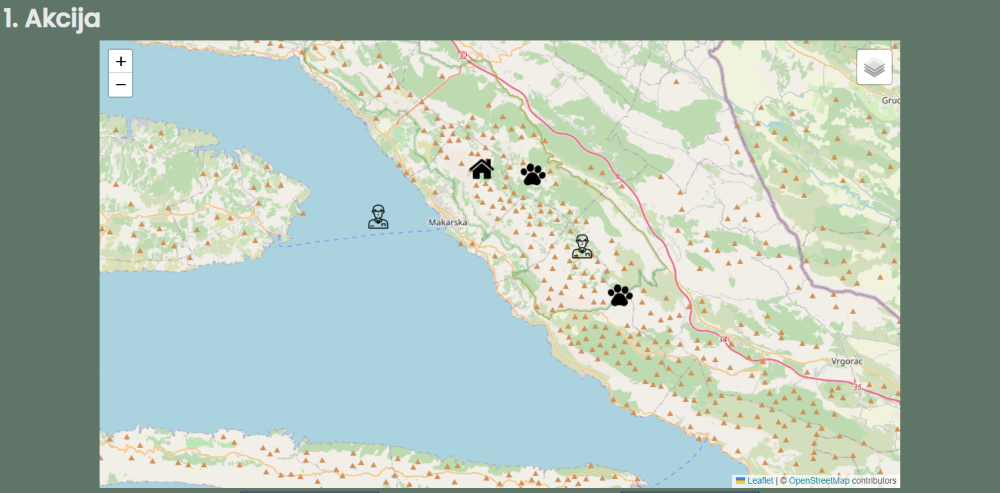
\includegraphics[scale=0.7]{slike/map_tracking.PNG} %veličina slike u odnosu na originalnu datoteku i pozicija slike
			\centering
			\caption{Primjer kartografskog prikaza trenutnih lokacija tragača i životinja}
			\label{fig:promjene}
		\end{figure}
		
		\begin{figure}[H]
			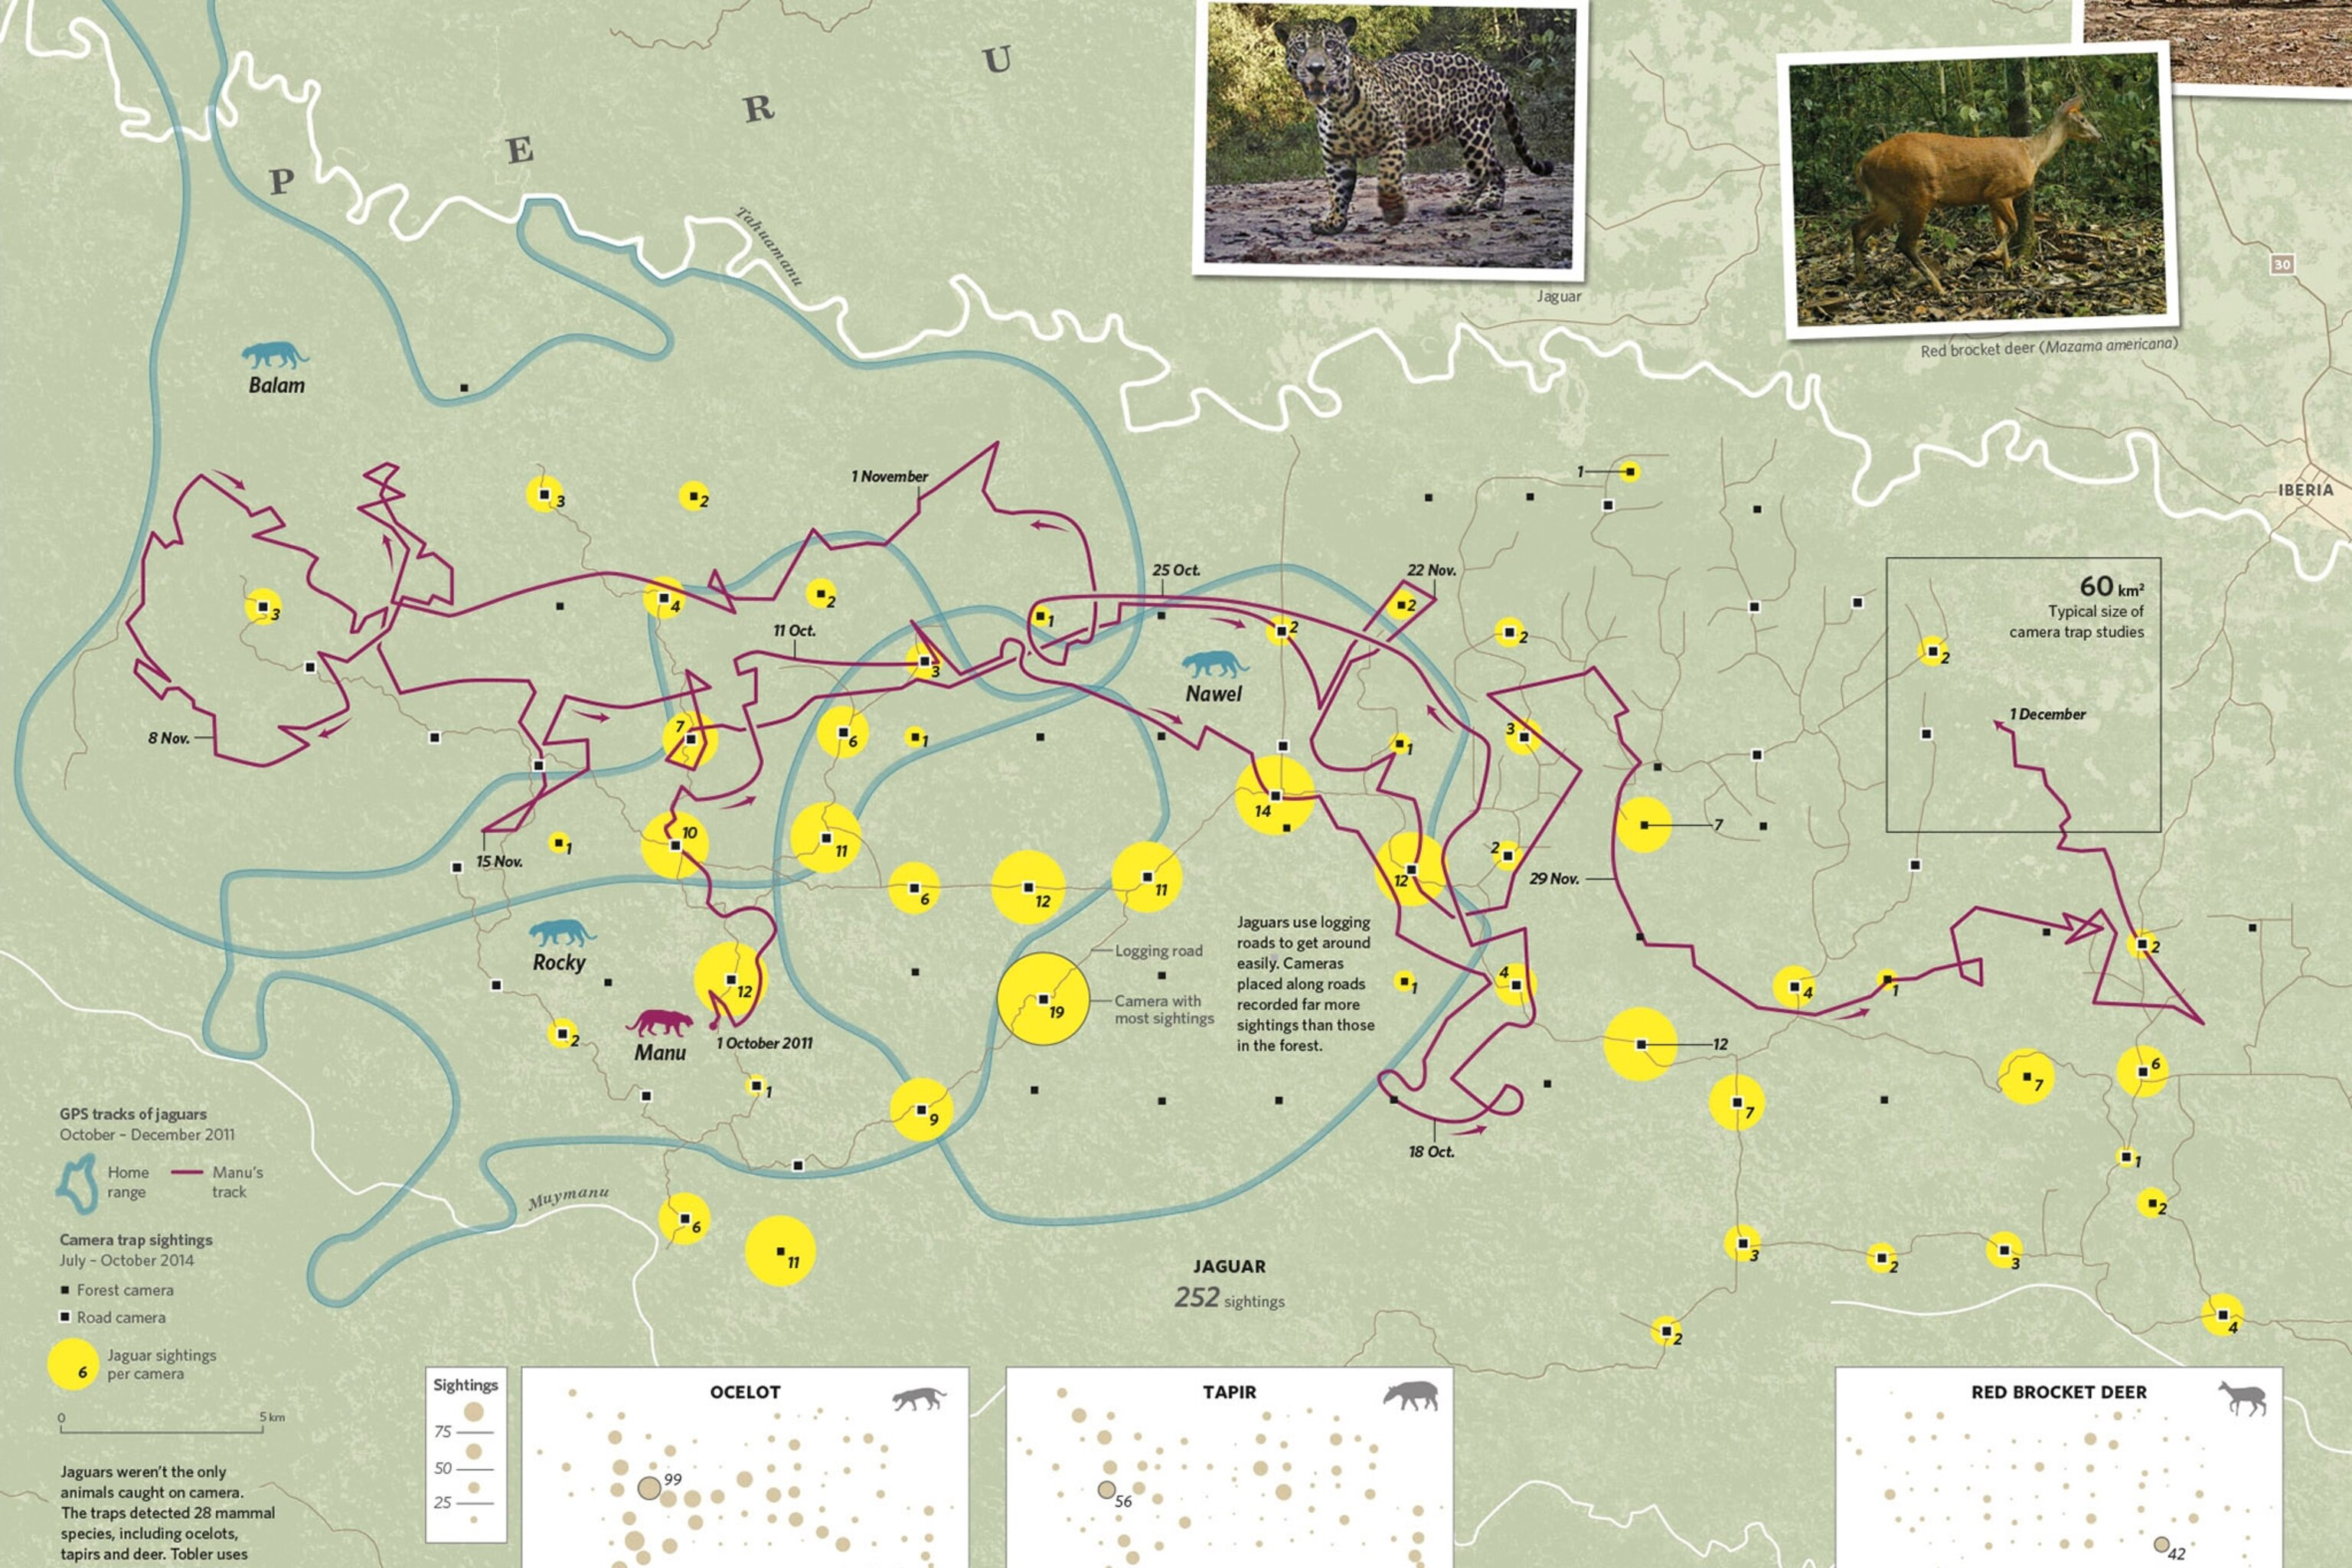
\includegraphics[scale=0.7]{slike/map_tracking2.PNG} %veličina slike u odnosu na originalnu datoteku i pozicija slike
			\centering
			\caption{Primjer kartografskog prikaza povijesnog kretanja tragača i životinja}
			\label{fig:promjene}
		\end{figure}
		
		\textbf{Tragač} će nakon same kreacije korisničkog računa biti slobodan i ostati takav dok ga neki voditelj ne doda u svoju postaju. Time mu se otvara mogućnost sudjelovanja u akcijama. Za vrijeme neke akcije, tragaču se na karti prikazuju zadaci koje treba obaviti, trenutna pozicija ostalih tragača aktivnih na istoj akciji, te trenutna pozicija praćenih životinja. Praćene životinje na sebi imaju gps uređaj koji aplikaciji odašilje svoju poziciju. O
		praćenim životinjama se zapisuju povijesni podaci gdje se nalazila, naziv vrste, slika i opis. Tragač može praćenoj životinji tijekom akcije ostaviti komentar. Također, tragač i istraživač mogu na karti ostaviti komentar za ostale sudionike u akciji.		
		
		\textbf{Administrator} sustava ima najveće ovlasti. On ima pregled svih poslanih zahtjeva za registraciju u ulozi istraživača ili voditelja postaje koje on mora potvrditi ili odbiti. Administrator ima pristup bazi s popisom svih registriranih korisnika i njihovih osobnih podataka te ih može mijenjati. On ujedno može i mijenjati ulogu dodijeljenu korisniku.
\vspace{12pt}

		Iako naša aplikacija ima mnogo specifičnih značajki usmjerenih praćenju životinja te ostalih korisnika, možemo pronaći slične značajke i u nekim drugim aplikacijama koje se bave praćenjem i kontekstu prirode i istraživanja. Primjeri uključuju aplikacije kao što su:
		
		\begin{packed_item}
		
			\item \textbf{Wildme}\linebreak
			Wildme je organizacija koja razvija tehnologiju prepoznavanja uzoraka koja omogućuje automatsko prepoznavanje pojedinaca u divljini putem fotografija i drugih podataka. Ima seriju online platformi unutar \textbf{Wildbook} projekta usmjerena na analizu i praćenje životinja. Time omogućuje zoolozima i istraživačima praćenje lakše praćenje jedinki.
\vspace{12pt}
			
			\item \textbf{iNaturalist}\linebreak
			iNaturalist je stranica koja omogucuje korisnicima dijeljenje svojih opažanja divljih biljka i životinja. Koristi se za indetifikaciju vrsta te obilježavanje raznolikosti vrsta u prirodi.
\vspace{12pt}
			
			\item \textbf{Movebank}\linebreak
			Movebank je stranica za praćenje migracija životinja. Koristi se za pohranu i analiziranje podataka o kretanju životinja označene GPS uređajima
\vspace{12pt}
			
			\item \textbf{Panthera}\linebreak
			Pantera je organizacija posvećena očuvanju divljih mačaka. Njihovi projekti uključuju praćenje životinja te suradnje s lokalnim zajednicama.
			
		\end{packed_item}
		
        \begin{figure}[H]
			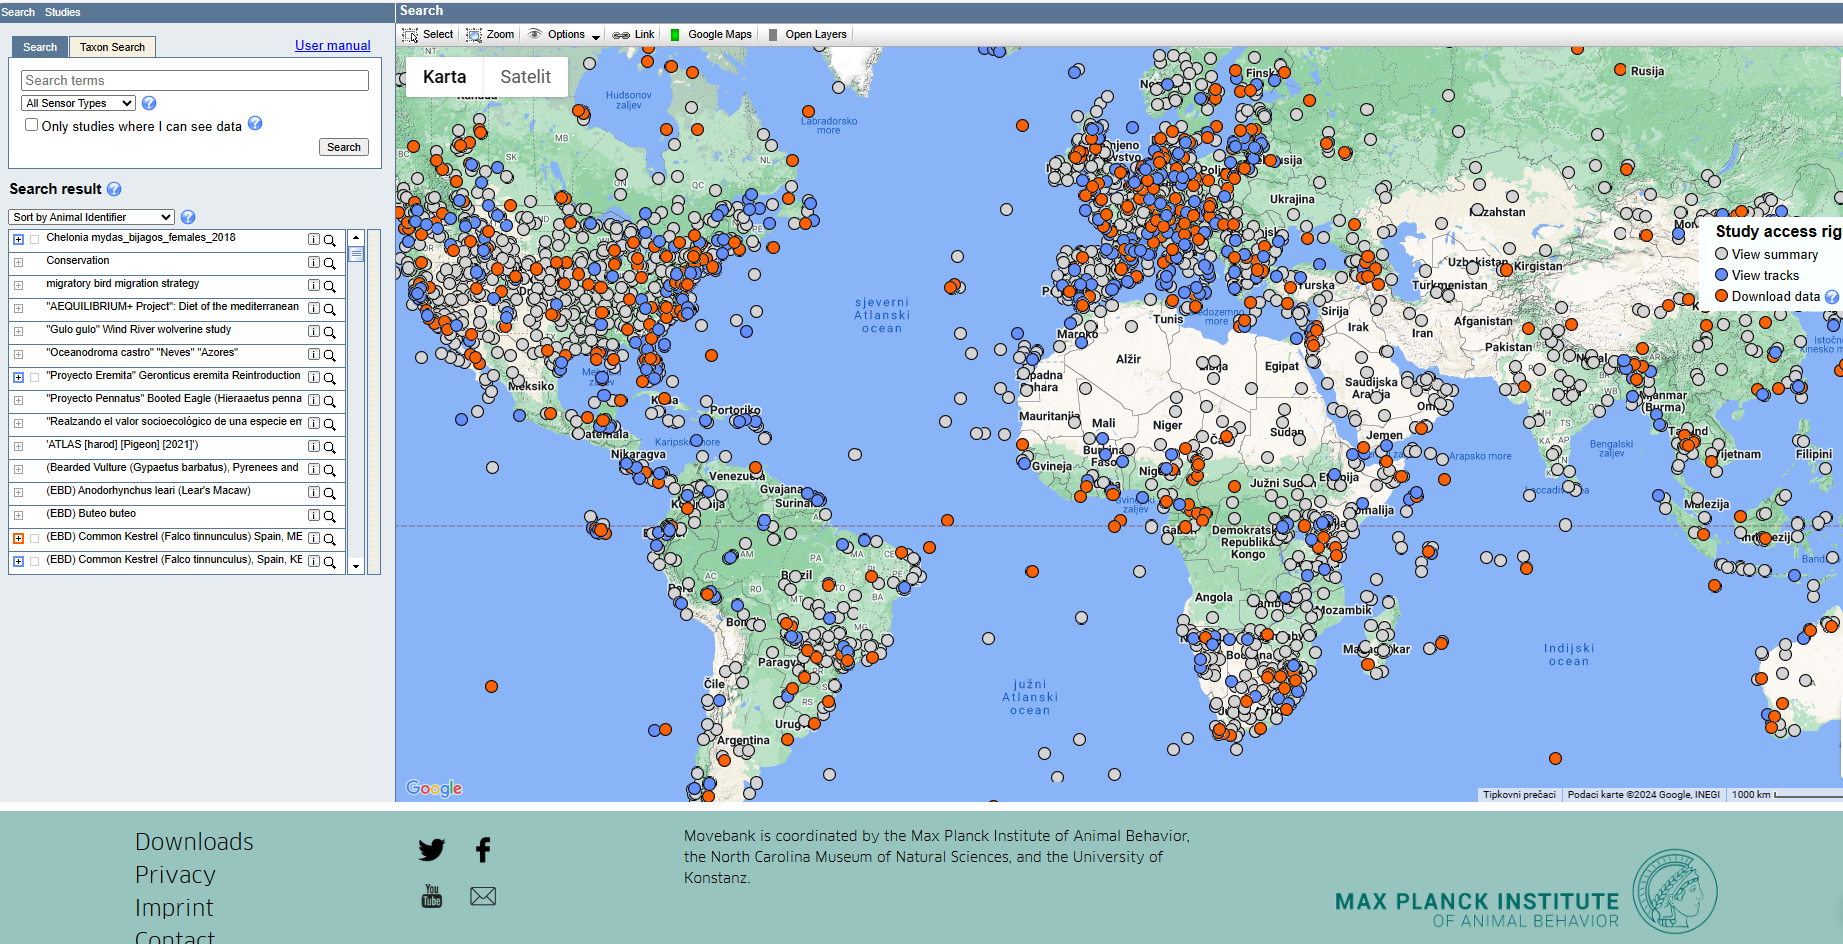
\includegraphics[scale=0.25]{slike/karta_movebank.PNG} %veličina slike u odnosu na originalnu datoteku i pozicija slike
			\centering
			\caption{Karta za praćenje životinja - Movebank}
			\label{fig:promjene}
		\end{figure}
		
		\begin{figure}[H]
		    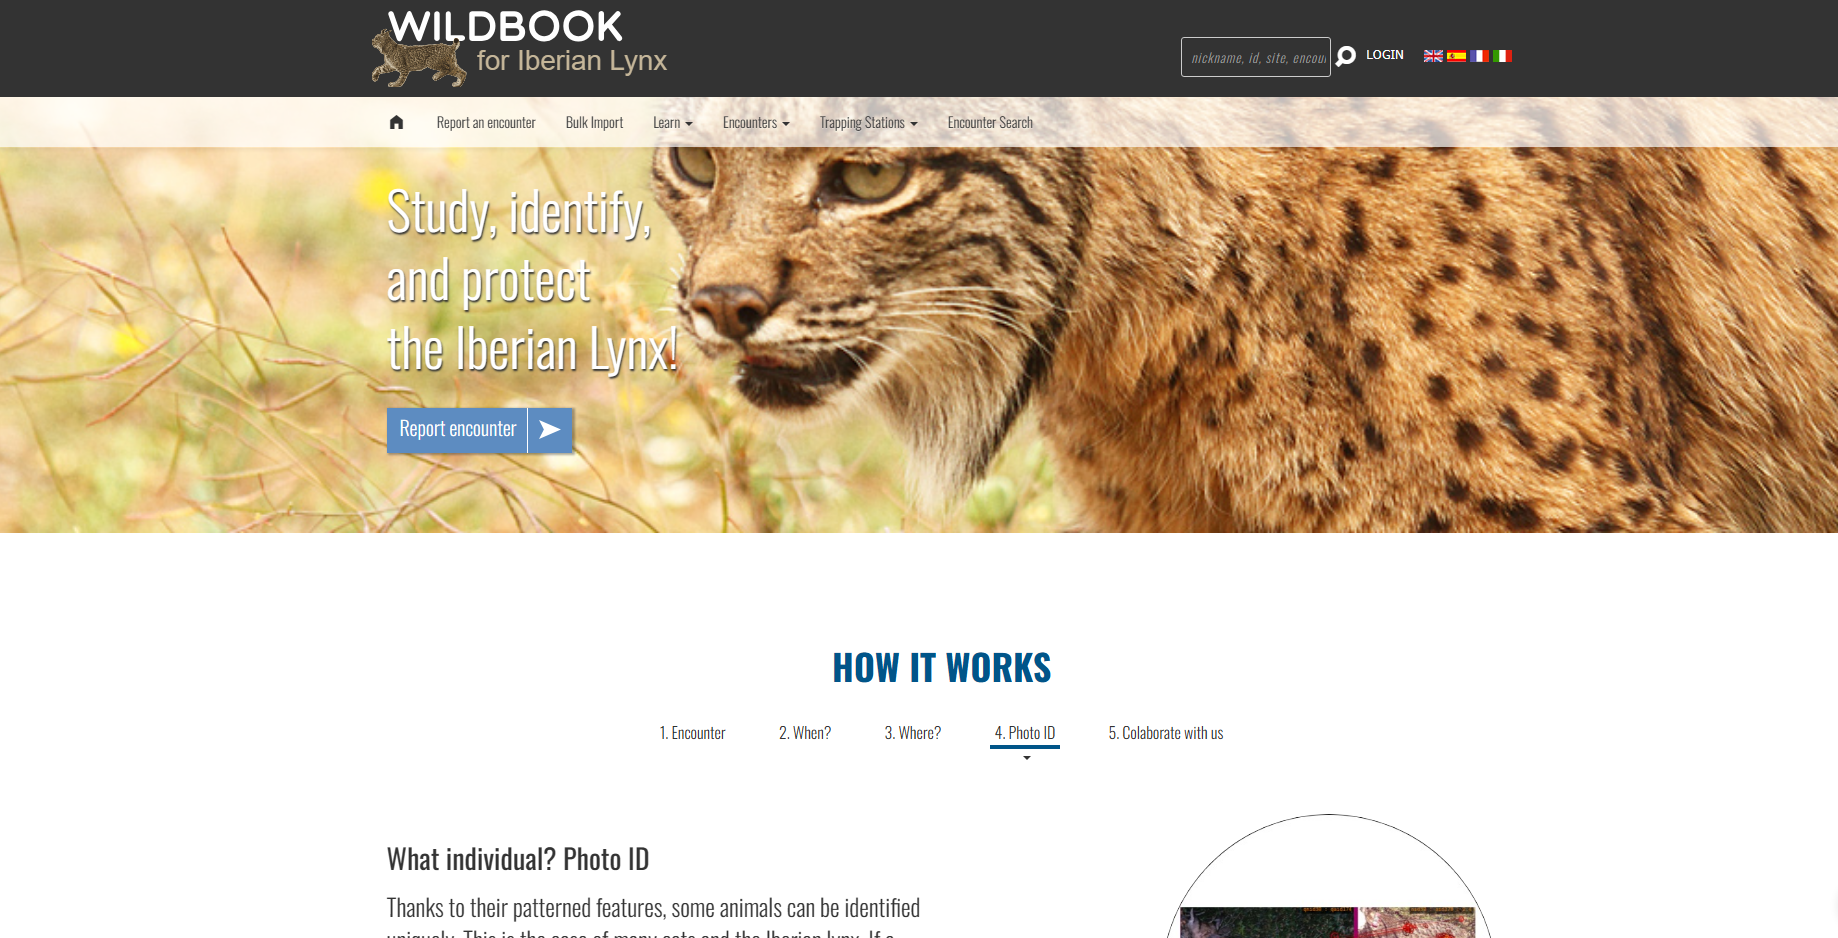
\includegraphics[scale=0.25]{slike/wildbook_ris.PNG} %veličina slike u odnosu na originalnu datoteku i pozicija slike
			\centering
			\caption{Wildbook za Pirenejskog risa}
			\label{fig:promjene}
		\end{figure}
		
		\begin{figure}[H]
			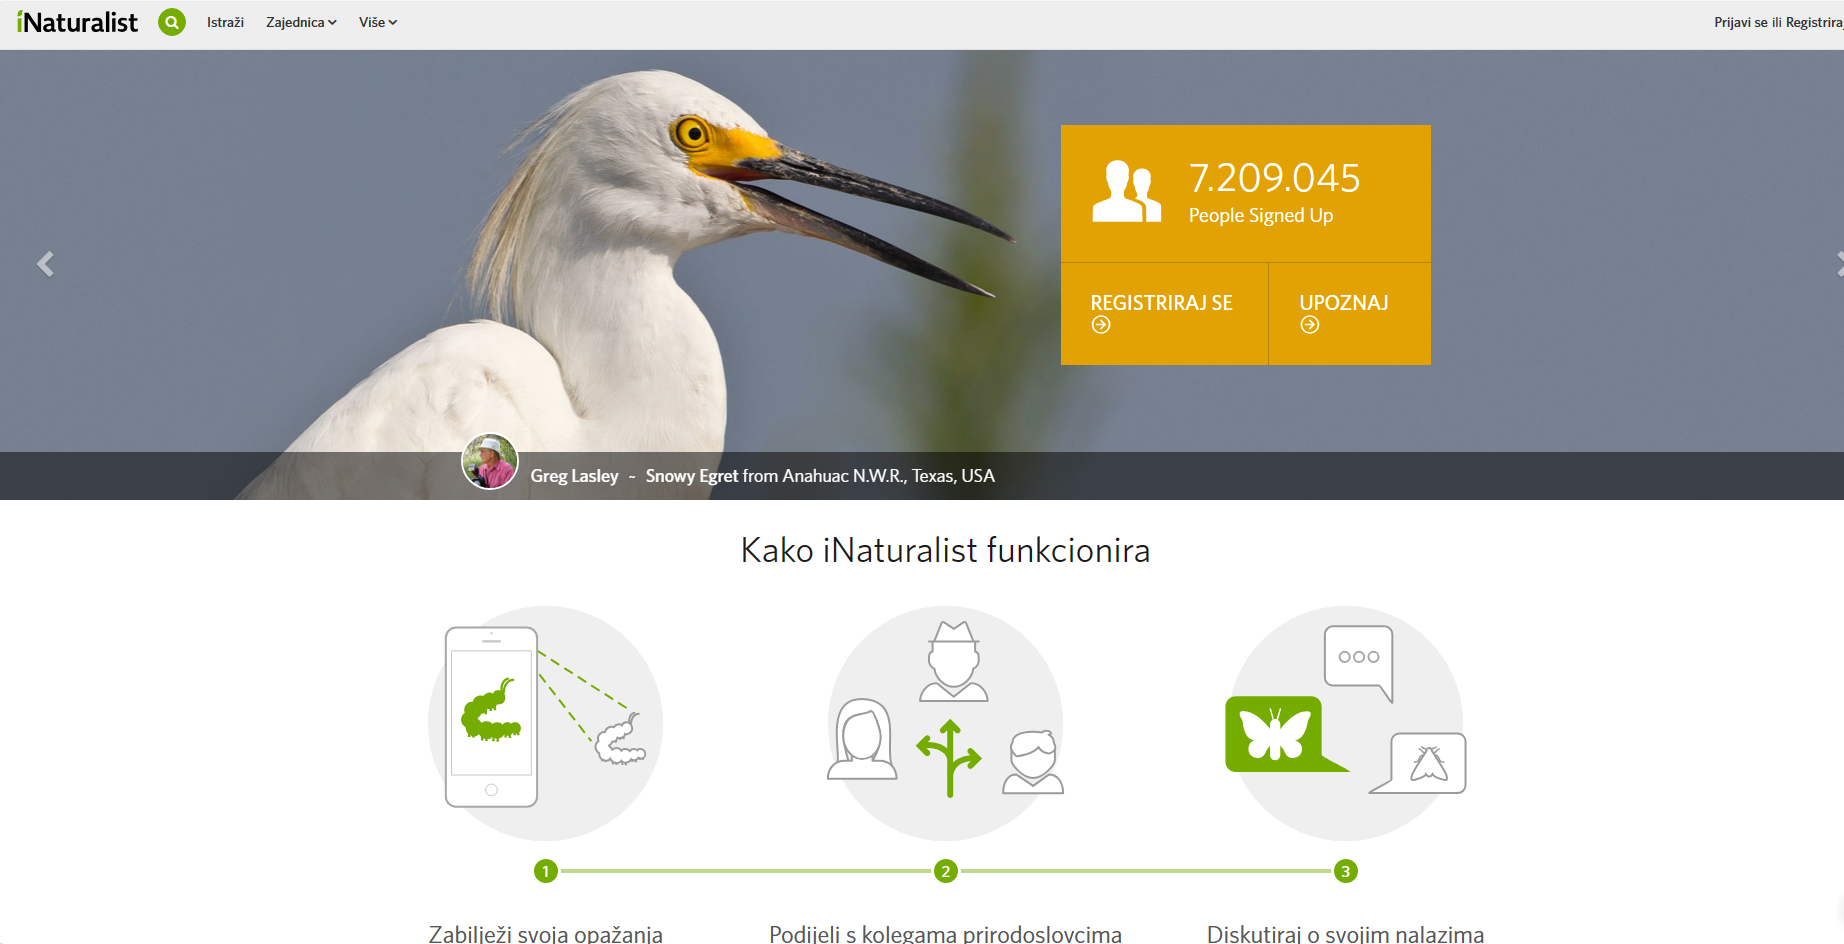
\includegraphics[scale=0.25]{slike/stranica_inaturalist.PNG} %veličina slike u odnosu na originalnu datoteku i pozicija slike
			\centering
			\caption{Stranica iNaturalist}
			\label{fig:promjene}
		\end{figure}
	\chapter{Specifikacija programske potpore}
		
	\section{Funkcionalni zahtjevi}
			
			\noindent \textbf{Dionici:}
			
			\begin{packed_enum}
				
				\item Naručitelj
				\item Korisnici
				\begin{enumerate}
					\item Voditelj postaje
					\item Istraživač
					\item Tragač
				\end{enumerate}		
				\item Administrator
				\item Razvojni tim 
				
			\end{packed_enum}
			
			\noindent \textbf{Aktori i njihovi funkcionalni zahtjevi:}
			
			
			\begin{packed_enum}
				\item  \underbar{Neregistrirani korisnik (inicijator) može:}
				
				\begin{packed_enum}
					
					\item poslati zahtjev za registraciju sa željenom ulogom za koju se prijavljuje
					
				\end{packed_enum}
				
			
				\item  \underbar{Voditelj postaje (inicijator) može:}
				
				\begin{packed_enum}
					
					\item dobiti pregled koji su tragači dio njegove postaje					
					\item dodati ili ukloniti tragače njegove postaje
					\item definirati na koji način su tragači osposobljeni izvoditi pretraživanje (pješke, dronom, automobilom, cross motorom, brodom ili helikopterom)
					\item odabrati konkretne tragače koji će sudjelovati u akciji
					\item ukloniti tragače s pojedine akcije po završetku njihova rada
					
				\end{packed_enum}
				
				\item  \underbar{Istraživač (inicijator) može:}
				
				\begin{packed_enum}
					
					\item dobiti pregled svih akcija koje je pokrenuo
					\item stvoriti nove akcije pretraživanja i praćenja s detaljima o određenim vrstama, jedinkama ili staništima za proučavanje
					\item poslati zahtjev za tragačima s opisom o potrebnim kvalifikacijama voditeljima postaja
					\item dobiti pregled koji tragači sudjeluju u akciji					
					\item preko karte tragačima pojedinačno zadati zadatke
					\item označiti da je neki tragač gotov sa svojim zadatkom
					\item ostaviti komentar za svaki zadatak
					\item bilježiti i vizualizirati staze kojima su tragači putovali i način kojim su se kretali u obliku toplinskih karata  
					\item odabrati da se za izradu interaktivnih karata koriste neka od idućih informacija: povijesne pozicije svih praćenih životinja, filtrirano po vrsti ili pojedinačno po jedinki te trenutne pozicije praćenih životinja 
					\item ostaviti komentar za ostale sudionike u akciji  
					
				\end{packed_enum}
				
				\item  \underbar{Tragač (inicijator) može:}
				
				\begin{packed_enum}
					 
					\item dobiti prikaz na karti zadataka koje treba obaviti, trenutne pozicije ostalih tragača aktivnih na istoj akciji, te trenutne pozicije praćenih životinja 
					\item ostaviti komentar za ostale sudionike u akciji
					\item ostaviti komentar o praćenoj životinji tijekom akcije 
					
				\end{packed_enum}
				
				\item  \underbar{Administrator (inicijator) može:}
				
				\begin{packed_enum}
					
					\item potvrditi istraživača i voditelja postaje tijekom registracije
					\item vidjeti popis svih registriranih korisnika i njihovih osobnih podataka  
					\item mijenjati osobne podatke svih registriranih korisnika te njihove uloge
					
				\end{packed_enum}
				
				\item  \underbar{Baza podataka (sudionik):}
				
				\begin{packed_enum}
					
					\item pohranjuje sve podatke o korisnicima i njihovim ovlastima 
					\item pohranjuje sve podatke o akcijama, lokacijama, životinjama i sl. 
					
				\end{packed_enum}
			\end{packed_enum}
			
			\eject 
			
			
				
			\subsection{Obrasci uporabe}
								
					\noindent \underbar{\textbf{UC1 - Registracija}}
					\begin{packed_item}
	
						\item \textbf{Glavni sudionik:} Neregistrirani korisnik
						\item \textbf{Cilj:} Stvoriti korisnički račun za pristup sustavu
						\item \textbf{Sudionici:} Baza podataka
						\item \textbf{Preduvjet:} -
						\item \textbf{Opis osnovnog tijeka:}
						
						\item[] \begin{packed_enum}
	
							\item Korisnik odabire opciju za registraciju  
							\item Korisnik unosi potrebne korisničke podatke (korisničko ime, fotografija, lozinka, ime, prezime i email adresa) te odabire željenu ulogu za koju se prijavljuje 
							\item Korisnik prima obavijest o uspješnoj/neuspješnoj registraciji
						\end{packed_enum}
						
						\item  \textbf{Opis mogućih odstupanja:}
						
						\item[] \begin{packed_item}
	
							\item[2.a] Odabir već zauzetog korisničkog imena i/ili e-maila, unos korisničkog podatka u nedozvoljenom formatu ili pružanje neispravnoga e-maila 
							\item[] \begin{packed_enum}
								
								\item Sustav obavještava korisnika o neuspjelom upisu i vraća ga na stranicu za registraciju 
								\item Korisnik mijenja potrebne podatke te završava unos ili odustaje od registracije 
								
							\end{packed_enum}
							\item[3.a] Administrator odbija registraciju korisnika koji se želi registrirati kao istraživač ili voditelj postaje
							\item[] \begin{packed_enum}
								
								\item Sustav obavještava korisnika o neuspjelom upisu i vraća ga na stranicu za registraciju 
								
							\end{packed_enum}
							
						\end{packed_item}
					\end{packed_item}
				
					\noindent \underbar{\textbf{UC2 - Prijava u sustav}}
					\begin{packed_item}
						
						\item \textbf{Glavni sudionik:} Korisnik
						\item \textbf{Cilj:} Dobiti pristup korisničkom sučelju 
						\item \textbf{Sudionici:} Baza podataka 
						\item \textbf{Preduvjet:} Korisnik ima registrirani korisnički račun
						\item \textbf{Opis osnovnog tijeka:}
						
						\item[] \begin{packed_enum}
							
							\item Unos korisničkog imena i lozinke 
							\item Potvrda o ispravnosti unesenih podataka 
							\item Pristup korisničkim funkcijama
						\end{packed_enum}
						
						\item  \textbf{Opis mogućih odstupanja:}
						
						\item[] \begin{packed_item}
							
							\item[2.a] Neispravno korisničko ime/lozinka
							\item[] \begin{packed_enum}
								
								\item Sustav obavještava korisnika o neuspjelom upisu i vraća ga na stranicu za registraciju
								
							\end{packed_enum}
							
						\end{packed_item}
					\end{packed_item}
					
					\noindent \underbar{\textbf{UC3 - Pregled osobnih podataka}}
					\begin{packed_item}
						
						\item \textbf{Glavni sudionik:} Korisnik
						\item \textbf{Cilj:} Pregledati osobne podatke
						\item \textbf{Sudionici:} Baza podataka
						\item \textbf{Preduvjet:} Korisnik je prijavljen
						\item \textbf{Opis osnovnog tijeka:}
						
						\item[] \begin{packed_enum}
							
							\item Korisnik odabire opciju ”Osobni podatci” 
							\item Sustav prikazuje osobne podatke korisnika
						\end{packed_enum}
					\end{packed_item}
					
					\noindent \underbar{\textbf{UC4 - Pregled članova postaje}}
					\begin{packed_item}
						
						\item \textbf{Glavni sudionik:} Voditelj postaje
						\item \textbf{Cilj:} Dobiti popis tragača koji su članovi postaje
						\item \textbf{Sudionici:} Baza podataka
						\item \textbf{Preduvjet:} Voditelj postaje je prijavljen
						\item \textbf{Opis osnovnog tijeka:}
						
						\item[] \begin{packed_enum}
							
							\item Voditelj bira opciju "Članovi postaje" 
							\item Sustav prikazuje popis tragača koji su članovi postaje
						\end{packed_enum}
					\end{packed_item}
					
					\noindent \underbar{\textbf{UC5 - Dodavanje tragača u postaju}}
					\begin{packed_item}
						
						\item \textbf{Glavni sudionik:} Voditelj postaje
						\item \textbf{Cilj:} Dodati slobodnog tragača među članove postaje
						\item \textbf{Sudionici:} Baza podataka, tragač
						\item \textbf{Preduvjet:} Voditelj postaje je prijavljen
						\item \textbf{Opis osnovnog tijeka:}
						
						\item[] \begin{packed_enum}
							
							\item Voditelj postaje bira opciju "Dodaj tragača u postaju" 
							\item Sustav prikazuje popis slobodnih tragača
							\item Voditelj odabire tragače koje želi dodijeliti svojoj postaji 
							\item Voditelj potvrđuje odabir 
							\item Sustav ažurira bazu podataka i dodjeljuje odabrane tragače postaji koju vodi voditelj
						\end{packed_enum}
						
						\item  \textbf{Opis mogućih odstupanja:}
						
						\item[] \begin{packed_item}
							
							\item[2.a] Ne postoji registrirani tragač koji već nije član neke postaje
							\item[] \begin{packed_enum}
								
								\item Sustav obavještava korisnika o nepostojanju slobodnih tragača
								
							\end{packed_enum}
							
						\end{packed_item}
					\end{packed_item}
					
					\eject
					
					\noindent \underbar{\textbf{UC6 - Uklanjanje tragača iz postaje}}
					\begin{packed_item}
						
						\item \textbf{Glavni sudionik:} Voditelj postaje
						\item \textbf{Cilj:} Ukloniti tragača iz članova postaje
						\item \textbf{Sudionici:} Baza podataka, tragač
						\item \textbf{Preduvjet:} Voditelj postaje je prijavljen i postoje tragači koji pripadaju njegovoj postaji
						\item \textbf{Opis osnovnog tijeka:}
						
						\item[] \begin{packed_enum}
							
							\item Voditelj postaje bira opciju "Ukloni tragača iz postaje" 
							\item Sustav prikazuje popis tragača koji su članovi postaje
							\item Voditelj odabire tragače koje želi ukloniti iz svoje postaje 
							\item Voditelj potvrđuje odabir 
							\item Sustav ažurira bazu podataka i odabrane tragače dodaje na listu slobodnih tragača
						\end{packed_enum}
						
						\item  \textbf{Opis mogućih odstupanja:}
						
						\item[] \begin{packed_item}
							
							\item[2.a] Ne postoji tragač koji je član postaje
							\item[] \begin{packed_enum}
								
								\item Sustav obavještava korisnika o nepostojanju tragača koji su članovi postaje
								
							\end{packed_enum}
					\end{packed_item}
					
					\noindent \underbar{\textbf{UC7 - Definiranje osposobljenosti tragača}}
					\begin{packed_item}
						
						\item \textbf{Glavni sudionik:} Voditelj postaje
						\item \textbf{Cilj:} Definirati na koji način su tragači osposobljeni izvoditi pretraživanje (pješke, dronom, automobilom, cross motorom, brodom ili helikopterom)
						\item \textbf{Sudionici:} Baza podataka, tragač
						\item \textbf{Preduvjet:} Voditelj je prijavljen i postoje tragači koji pripadaju njegovoj postaji
						\item \textbf{Opis osnovnog tijeka:}
						
						\item[] \begin{packed_enum}
							
							\item Sustav prikazuje popis tragača koji su članovi postaje
							\item Voditelj postaje odabire tragača 
							\item Voditelj odabire opciju "Definiraj osposobljenost tragača" 
							\item Voditelj odabire koja osposobljenja za način pretraživanja ima tragač
							\item Voditelj potvrđuje odabir 
							\item Sustav ažurira bazu podataka s odabranim načinima pretraživanja
						\end{packed_enum}
					\end{packed_item}
					
					\noindent \underbar{\textbf{UC8 - Pregled zahtjeva za tragačima}}
					\begin{packed_item}
						
						\item \textbf{Glavni sudionik:} Voditelj postaje
						\item \textbf{Cilj:} Dobiti popis pristiglih zahtjeva za alociranje tragača za sudjelovanje u akciji
						\item \textbf{Sudionici:} Baza podataka
						\item \textbf{Preduvjet:} Voditelj je prijavljen
						\item \textbf{Opis osnovnog tijeka:}
						
						\item[] \begin{packed_enum}
							
							\item Voditelj odabire opciju "Pristigli zahtjevi"
							\item Sustav prikazuje popis pristiglih zahtjeva za alociranje tragača za sudjelovanje u akciji
						\end{packed_enum}
						
						\item  \textbf{Opis mogućih odstupanja:}
						
						\item[] \begin{packed_item}
							
							\item[2.a] Nije pristigao niti jedan zahtjev
							\item[] \begin{packed_enum}
								
								\item Sustav obavještava korisnika o nepostojanju pristiglih zahtjeva
								
							\end{packed_enum}
					\end{packed_item}
					
					
					\noindent \underbar{\textbf{UC9 - Odabir tragača za akciju}}
					\begin{packed_item}
						
						\item \textbf{Glavni sudionik:} Voditelj postaje
						\item \textbf{Cilj:} Odabrati koji tragači će sudjelovati u nekoj akciji
						\item \textbf{Sudionici:} Baza podataka, tragač
						\item \textbf{Preduvjet:} Voditelj je prijavljen i primio je barem jedan zahtjev za alociranjem tragača za sudjelovanje u akciji
						\item \textbf{Opis osnovnog tijeka:}
						
						\item[] \begin{packed_enum}
							
							\item Sustav prikazuje zahtjev za alociranjem tragača za sudjelovanje u akciji
							\item Voditelj postaje odabire opciju "Odaberi tragače za akciju"
							\item Sustav prikazuje popis raspoloživih tragača
							\item Voditelj odabire tragača
							\item Voditelj potvrđuje odabir
							\item Sustav ažurira bazu podataka i dodjeljuje odabrane tragače akciji 
						\end{packed_enum}
						
						\item  \textbf{Opis mogućih odstupanja:}
						
						\item[] \begin{packed_item}
							
							\item[2.a] Nema raspoloživih tragača
							\item[] \begin{packed_enum}
								
								\item Sustav obavještava voditelj o nedostatku raspoloživih tragača								
							\end{packed_enum}
							
						\end{packed_item}
						
					\end{packed_item}
					
					\noindent \underbar{\textbf{UC10 - Uklanjanje tragača s akcije}}
					\begin{packed_item}
						
						\item \textbf{Glavni sudionik:} Voditelj postaje
						\item \textbf{Cilj:} Odabrati koji tragači će sudjelovati u nekoj akciji
						\item \textbf{Sudionici:} Baza podataka, tragač
						\item \textbf{Preduvjet:} Voditelj je prijavljen i tragač sudjeluje u nekoj akciji
						\item \textbf{Opis osnovnog tijeka:}
						
						\item[] \begin{packed_enum}
							
							\item Sustav prikazuje popis tragača koji su članovi postaje 
							\item Voditelj odabire tragača kojeg želi ukloniti s neke akcije
							\item Voditelj odabire opciju "Ukloni s akcije"
							\item Voditelj potvrđuje odabir
							\item Sustav ažurira bazu podataka i vraća tragača na popis raspoloživih tragača
						\end{packed_enum}
						
						\item  \textbf{Opis mogućih odstupanja:}
						
						\item[] \begin{packed_item}
							
							\item[3.a] Tragač nije završio sa zadatkom na akciji
							\item[] \begin{packed_enum}
								
								\item Sustav obavještava voditelja da mu nije dopušteno ukloniti tragača s akcije			
							\end{packed_enum}
							
						\end{packed_item}
						
					\end{packed_item}
					
					\noindent \underbar{\textbf{UC11 - Pregled akcija}}
					\begin{packed_item}
						
						\item \textbf{Glavni sudionik:} Istraživač
						\item \textbf{Cilj:} Dobiti popis akcija u kojima istraživač sudjeluje
						\item \textbf{Sudionici:} Baza podataka
						\item \textbf{Preduvjet:} Istraživač je prijavljen
						\item \textbf{Opis osnovnog tijeka:}
						
						\item[] \begin{packed_enum}
							
							\item Istraživač odabire opciju "Moje akcije" 
							\item Sustav prikazuje popis akcija u kojima istraživač sudjeluje
						\end{packed_enum}
					\end{packed_item}
					
					\noindent \underbar{\textbf{UC12 - Stvaranje novih akcija}}
					\begin{packed_item}
						
						\item \textbf{Glavni sudionik:} Istraživač
						\item \textbf{Cilj:} Stvoriti novu akciju pretraživanja i praćenja s detaljima o određenim vrstama, jedinkama ili staništima za proučavanje
						\item \textbf{Sudionici:} Baza podataka
						\item \textbf{Preduvjet:} Istraživač je prijavljen
						\item \textbf{Opis osnovnog tijeka:}
						
						\item[] \begin{packed_enum}
							
							\item Istraživač odabire opciju "Stvori novu akciju" 
							\item Sustav prikazuje obrazac za unos detalja o akciji 
							\item Istraživač unosi tražene podatke 
							\item Istraživač potvrđuje unos 
							\item Sustav ažurira bazu podataka s novom akcijom 
						\end{packed_enum}
					\end{packed_item}
					
					\noindent \underbar{\textbf{UC13 - Slanje zahtjeva za tragačima}}
					\begin{packed_item}
						
						\item \textbf{Glavni sudionik:} Istraživač
						\item \textbf{Cilj:} Poslati zahtjev za tragačima s opisom o potrebnim kvalifikacijama voditeljima postaja
						\item \textbf{Sudionici:} Baza podataka, voditelj postaje
						\item \textbf{Preduvjet:} Istraživač je prijavljen i postoji barem jedan voditelj postaje s tragačima u svojoj postaji
						\item \textbf{Opis osnovnog tijeka:}
						
						\item[] \begin{packed_enum}
							
							\item Istraživač odabire opciju "Pošalji zahtjev za tragačima" 
							\item Sustav prikazuje obrazac za unos detalja o zahtjevu (kvalifikacije, broj tragača, itd.) 
							\item Istraživač unosi tražene podatke 
							\item Istraživač odabire postaju kojoj želi poslati zahtjev
							\item Istraživač potvrđuje slanje zahtjeva
							\item Sustav ažurira bazu podataka s poslanim zahtjevom
						\end{packed_enum}
					\end{packed_item}
					
					\noindent \underbar{\textbf{UC14 - Pregled članova akcije}}
					\begin{packed_item}
						
						\item \textbf{Glavni sudionik:} Istraživač
						\item \textbf{Cilj:} Dobiti popis tragača koji sudjeluju u akciji
						\item \textbf{Sudionici:} Baza podataka
						\item \textbf{Preduvjet:} Istraživač je prijavljen
						\item \textbf{Opis osnovnog tijeka:}
						
						\item[] \begin{packed_enum}
							
							\item Sustav prikazuje popis akcija u kojima istraživač sudjeluje
							\item Istraživač odabire akciju
							\item Istraživač odabire opciju "Članovi akcije"
							\item Sustav prikazuje popis tragača koji sudjeluju u akciji
						\end{packed_enum}
					\end{packed_item}
					
					\noindent \underbar{\textbf{UC15 - Dodjela zadatka tragaču}}
					\begin{packed_item}
						
						\item \textbf{Glavni sudionik:} Istraživač
						\item \textbf{Cilj:} Dodijeliti određen zadatak akcije nekom tragaču koji sudjeluje u akciji
						\item \textbf{Sudionici:} Baza podataka, tragač
						\item \textbf{Preduvjet:} Istraživač je prijavljen i postoji barem jedan tragač koji sudjeluje u akciji
						\item \textbf{Opis osnovnog tijeka:}
						
						\item[] \begin{packed_enum}
							
							\item Sustav prikazuje popis tragača koji sudjeluju u akciji
							\item Istraživač odabire tragača kojem želi dodijeliti zadatak
							\item Istraživač odabire opciju "Dodijeli zadatak tragaču" 
							\item Sustav prikazuje kartu
							\item Istraživač odabire rutu i odredišnu lokaciju zadatka
							\item Istraživač odabire koji uređaj želi da bude postavljen(kamera ili uređaj za praćenje) 
							\item Istraživač potvrđuje dodjelu zadatka 
							\item Sustav ažurira bazu podataka s dodijeljenim zadatkom tragaču 				
						\end{packed_enum}
					\end{packed_item}
					
					\eject
					
					\noindent \underbar{\textbf{UC16 - Pregled zadataka}}
					\begin{packed_item}
						
						\item \textbf{Glavni sudionik:} Istraživač
						\item \textbf{Cilj:} Dobiti popis zadataka zadanih u akciji
						\item \textbf{Sudionici:} Baza podataka
						\item \textbf{Preduvjet:} Istraživač je prijavljen
						\item \textbf{Opis osnovnog tijeka:}
						
						\item[] \begin{packed_enum}
							
							\item Sustav prikazuje popis akcija u kojima istraživač sudjeluje
							\item Istraživač odabire akciju
							\item Istraživač odabire opciju "Pregled zadataka"
							\item Sustav prikazuje popis zadataka koje je istraživač dodijelio
						\end{packed_enum}
					\end{packed_item}
					
					\noindent \underbar{\textbf{UC17 - Ostavljanje komentara za zadatak}}
					\begin{packed_item}
						
						\item \textbf{Glavni sudionik:} Istraživač
						\item \textbf{Cilj:} Ostaviti komentar za neki zadatak
						\item \textbf{Sudionici:} Baza podataka
						\item \textbf{Preduvjet:} Istraživač je prijavljen i dodijelio je barem jedan zadatak
						\item \textbf{Opis osnovnog tijeka:}
						
						\item[] \begin{packed_enum}
							
							\item Sustav prikazuje popis zadataka koje je istraživač dodijelio
							\item Istraživač odabire zadatak
							\item Istraživač odabire opciju "Ostavi komentar" 
							\item Istraživač unosi željeni komentar 
							\item Istraživač potvrđuje unos 
							\item Sustav ažurira bazu podataka s novim komentarom za zadatak 
						\end{packed_enum}
					\end{packed_item}
					
					\noindent \underbar{\textbf{UC18 - Dovršavanje zadatka}}
					\begin{packed_item}
						
						\item \textbf{Glavni sudionik:} Istraživač
						\item \textbf{Cilj:} Označiti da je neki zadatak dovršen
						\item \textbf{Sudionici:} Baza podataka
						\item \textbf{Preduvjet:} Istraživač je prijavljen i dodijelio je barem jedan zadatak
						\item \textbf{Opis osnovnog tijeka:}
						
						\item[] \begin{packed_enum}
							
							\item Sustav prikazuje popis zadataka koje je istraživač dodijelio
							\item Istraživač odabire zadatak
							\item Istraživač odabire opciju "Označi dovršenim" 
							\item Istraživač potvrđuje unos 
							\item Sustav ažurira bazu podataka s oznakom da je tragač završio zadatak 
						\end{packed_enum}
					\end{packed_item}
					
					\eject
					
					\noindent \underbar{\textbf{UC19 - Prikaz interaktivne karte}}
					\begin{packed_item}
						
						\item \textbf{Glavni sudionik:} Istraživač
						\item \textbf{Cilj:} Stvoriti interaktivnu kartu
						\item \textbf{Sudionici:} Baza podataka
						\item \textbf{Preduvjet:} Istraživač je prijavljen
						\item \textbf{Opis osnovnog tijeka:}
						
						\item[] \begin{packed_enum}
							
							\item Istraživač odabire opciju "Karta" 
							\item Sustav učitava kartu s posljednjim spremljenim promjenama
						\end{packed_enum}
					\end{packed_item}
					
					\noindent \underbar{\textbf{UC20 - Uređivanje interaktivne karte}}
					\begin{packed_item}
						
						\item \textbf{Glavni sudionik:} Istraživač
						\item \textbf{Cilj:} Stvoriti interaktivnu kartu
						\item \textbf{Sudionici:} Baza podataka
						\item \textbf{Preduvjet:} Istraživač je prijavljen
						\item \textbf{Opis osnovnog tijeka:}
						
						\item[] \begin{packed_enum}
							
							\item Istraživač odabire opciju "Uredi kartu"
							\item Sustav prikazuje opcije informacija koje mogu biti prikazane na karti
							\item Istraživač uređuje kartu prema svojim potrebama
							\item Istraživač potvrđuje promjene
							\item Sustav pohranjuje interaktivnu kartu u bazu podataka 
						\end{packed_enum}
					\end{packed_item}
					
					\noindent \underbar{\textbf{UC21 - Ostavljanje komentara na karti}}
					\begin{packed_item}
						
						\item \textbf{Glavni sudionik:} Istraživač, tragač
						\item \textbf{Cilj:} Ostaviti komentar na karti drugim sudionicima akcije
						\item \textbf{Sudionici:} Baza podataka
						\item \textbf{Preduvjet:} Istraživač ili tragač je prijavljen i sudjeluje u akciji
						\item \textbf{Opis osnovnog tijeka:}
						
						\item[] \begin{packed_enum}
							
							\item Sustav prikazuje kartu
							\item Istraživač ili tragač odabire opciju "Ostavi komentar" 
							\item Istraživač ili tragač unosi željeni komentar 
							\item Istraživač ili tragač potvrđuje unos 
							\item Sustav ažurira bazu podataka s novim komentarom za sudionike akcije 
						\end{packed_enum}
					\end{packed_item}
					
					\noindent \underbar{\textbf{UC22 - Ostavljanje komentara za praćenu životinju}}
					\begin{packed_item}
						
						\item \textbf{Glavni sudionik:} Tragač
						\item \textbf{Cilj:} Ostaviti komentar praćenoj životinji 
						\item \textbf{Sudionici:} Baza podataka
						\item \textbf{Preduvjet:} Tragač je prijavljen i sudjeluje u akciji
						\item \textbf{Opis osnovnog tijeka:}
						
						\item[] \begin{packed_enum}
							
							\item Tragač odabire opciju "Ostavi komentar za životinju" 
							\item Sustav prikazuje polje za unos komentara 
							\item Tragač unosi željeni komentar 
							\item Tragač potvrđuje unos 
							\item Sustav ažurira bazu podataka s novim komentarom za praćenu životinju 
						\end{packed_enum}
					\end{packed_item}
					
					\noindent \underbar{\textbf{UC23 - Pregled karte}}
					\begin{packed_item}
						
						\item \textbf{Glavni sudionik:} Tragač
						\item \textbf{Cilj:} Pristupiti karti za pregled zadataka koje treba obaviti, trenutne pozicije ostalih tragača aktivnih na istoj akciji, te trenutne pozicije praćenih životinja
						\item \textbf{Sudionici:} Baza podataka
						\item \textbf{Preduvjet:} Tragač je prijavljen i sudjeluje u akciji 
						\item \textbf{Opis osnovnog tijeka:}
						
						\item[] \begin{packed_enum}
							
							\item Tragač odabire opciju "Karta" 
							\item Sustav prikazuje kartu s označenim zadacima, pozicijama tragača i praćenih životinja 
							\item Tragač može interaktivno pregledavati kartu i pratiti informacije o akciji
						\end{packed_enum}
					\end{packed_item}
					
					\noindent \underbar{\textbf{UC24 - Pregled zahtjeva za registracijom}}
					\begin{packed_item}
						
						\item \textbf{Glavni sudionik:} Administrator
						\item \textbf{Cilj:} Dobiti popis svih pristiglih zahtjeva za registracijom u ulozi voditelja postaje ili istraživača
						\item \textbf{Sudionici:} Baza podataka
						\item \textbf{Preduvjet:} Korisnik je registriran i dodijeljena su mu prava administratora te postoji barem jedan zahtjev za registracijom u ulozi voditelja ili istraživača
						\item \textbf{Opis osnovnog tijeka:}
						
						\item[] \begin{packed_enum}
							
							\item Administrator odabire opciju "Pristigli zahtjevi"
							\item Sustav prikazuje popis pristiglih zahtjeva za registraciju u u ulozi voditelja postaje ili istraživača 
						\end{packed_enum}
					\end{packed_item}
					
					\eject
					
					\noindent \underbar{\textbf{UC25 - Potvrda registracije}}
					\begin{packed_item}
						
						\item \textbf{Glavni sudionik:} Administrator
						\item \textbf{Cilj:} Potvrditi/odbiti registraciju korisnika koji se želi registrirati kao istraživač ili voditelj postaje
						\item \textbf{Sudionici:} Baza podataka, neregistrirani korisnik
						\item \textbf{Preduvjet:} Administrator je registriran 
						\item \textbf{Opis osnovnog tijeka:}
						
						\item[] \begin{packed_enum}
							
							\item Sustav prikazuje popis pristiglih zahtjeva za registraciju u ulozi voditelja postaje ili istraživača
							\item Administrator odabire zahtjev 
							\item Administrator odabire opciju "Potvrdi" ili "Odbij"
							\item Ako administrator odabere opciju potvrdi, sustav ažurira bazu podataka s novim korisnikom
						\end{packed_enum}
					\end{packed_item}
					
					\noindent \underbar{\textbf{UC26 - Pregled svih korisnika}}
					\begin{packed_item}
						
						\item \textbf{Glavni sudionik:} Administrator
						\item \textbf{Cilj:} Pregledati sve registrirane korisnike i njihove osobne podatke
						\item \textbf{Sudionici:} Baza podataka
						\item \textbf{Preduvjet:} Administrator je registriran
						\item \textbf{Opis osnovnog tijeka:}
						
						\item[] \begin{packed_enum}
							
							\item Administrator odabire opciju "Pregled korisnika" 
							\item Sustav prikazuje popis svih registriranih korisnika i njihovih osobnih podataka
						\end{packed_enum}
					\end{packed_item}
					
					\noindent \underbar{\textbf{UC27 - Promjena osobnih podataka korisnika}}
					\begin{packed_item}
						
						\item \textbf{Glavni sudionik:} Administrator
						\item \textbf{Cilj:} Promijeniti osobne podatke korisnika
						\item \textbf{Sudionici:} Baza podataka, korisnik 
						\item \textbf{Preduvjet:} Administrator je registriran te postoji barem jedan registrirani korisnik
						\item \textbf{Opis osnovnog tijeka:}
						
						\item[] \begin{packed_enum}
							
							\item Sustav prikazuje popis svih registriranih korisnika i njihovih osobnih podataka
							\item Administrator bira korisnika
							\item Administrator odabire opciju "Uredi podatke"
							\item Administrator radi promjene
							\item Administrator sprema promjene 
							\item Sustav ažurira bazu podataka					
						\end{packed_enum}
						
						\item  \textbf{Opis mogućih odstupanja:}
						
						\item[] \begin{packed_item}
							
							\item[5.a] Administrator promijeni podatke, ali ne odabere opciju ”Spremi promjenu” 
							\item[] \begin{packed_enum}
								
								\item Sustav obavještava administratora da nije spremio podatke prije izlaska iz prozora
								
							\end{packed_enum}
							
						\end{packed_item}
					\end{packed_item}
					
					\noindent \underbar{\textbf{UC28 - Promjena uloge korisnika}}
					\begin{packed_item}
						
						\item \textbf{Glavni sudionik:} Administrator
						\item \textbf{Cilj:} Promijeniti osobne podatke korisnika
						\item \textbf{Sudionici:} Baza podataka, korisnik
						\item \textbf{Preduvjet:} Korisnik je registriran i dodijeljena su mu prava administratora te postoji barem jedan registrirani korisnik
						\item \textbf{Opis osnovnog tijeka:}
						
						\item[] \begin{packed_enum}
							
							\item Sustav prikazuje popis svih registriranih korisnika i njihovih osobnih podataka
							\item Administrator bira korisnika
							\item Administrator odabire opciju "Promijeni ulogu"
							\item Administrator odabire novu ulogu korisnika
							\item Administrator sprema promjene 
							\item Sustav ažurira bazu podataka					
						\end{packed_enum}
						
						\item  \textbf{Opis mogućih odstupanja:}
						
						\item[] \begin{packed_item}
							
							\item[4.a] Administrator promijeni ulogu voditelja postaje
							\item[] \begin{packed_enum}
								
								\item Sustav obavještava administratora da mora odabrati novog voditelja postaje i prikazuje mu popis članova postaje
								\item Administrator bira tragača kojem će promijeniti ulogu u voditelja postaje
								
							\end{packed_enum}
							
							\item[4.b] Administrator promijeni ulogu u voditelja postaje
							\item[] \begin{packed_enum}
								
								\item Sustav obavještava administratora da će dosadašnjem voditelju postaje uloga biti promjena u tragača
								
							\end{packed_enum}
							
						\end{packed_item}
					\end{packed_item}
					
				\eject
					
					
				\subsubsection{Dijagrami obrazaca uporabe}
					\begin{figure}[H]
						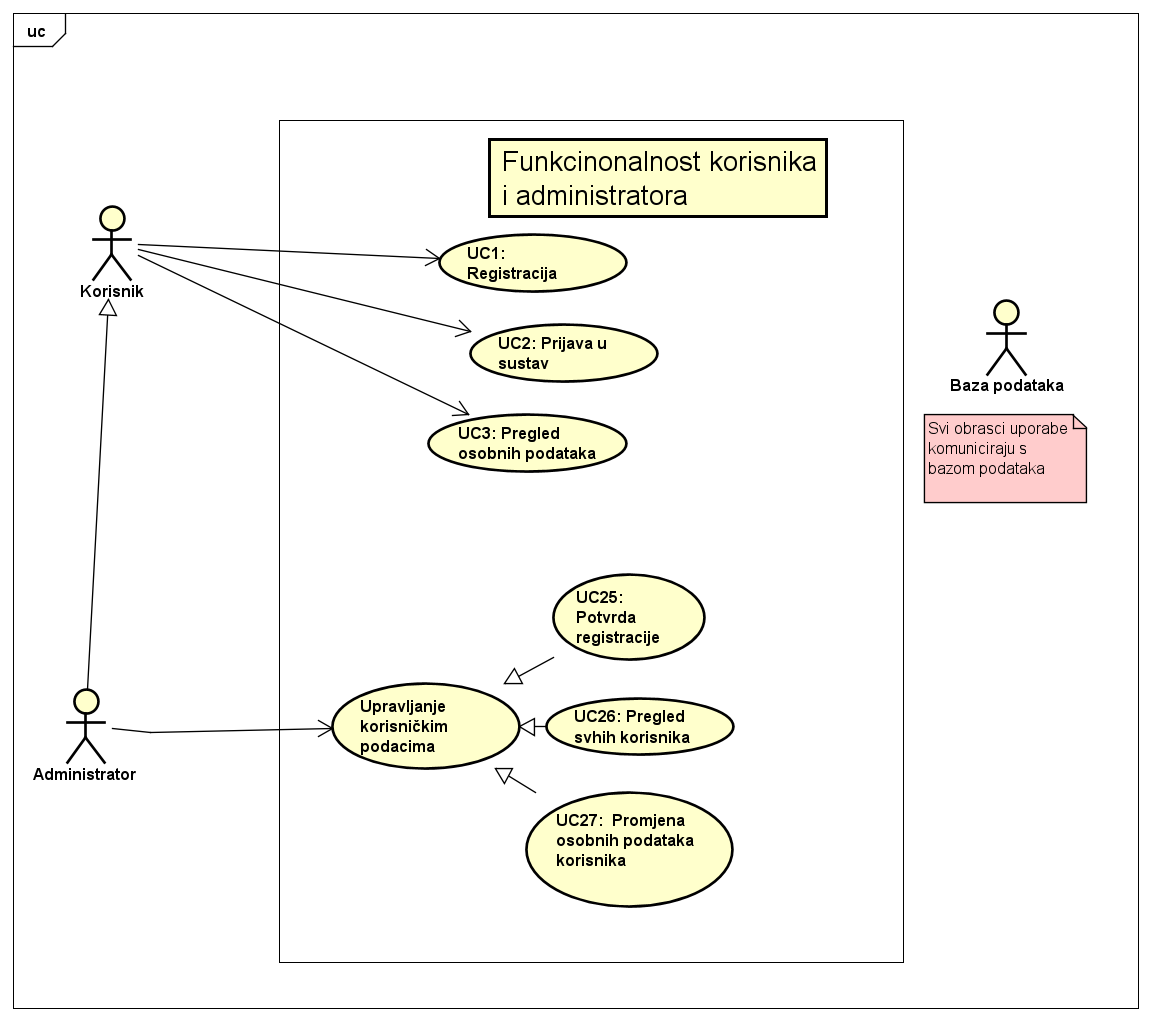
\includegraphics[scale=0.4]{dijagrami/Korisnik-admin_dijagram.png} 
						\centering
						\caption{Dijagram obrasca uporabe, funkcionalnost korisnika i administratora}
						\label{fig:promjene}
					\end{figure}	
					
					\begin{figure}[H]
						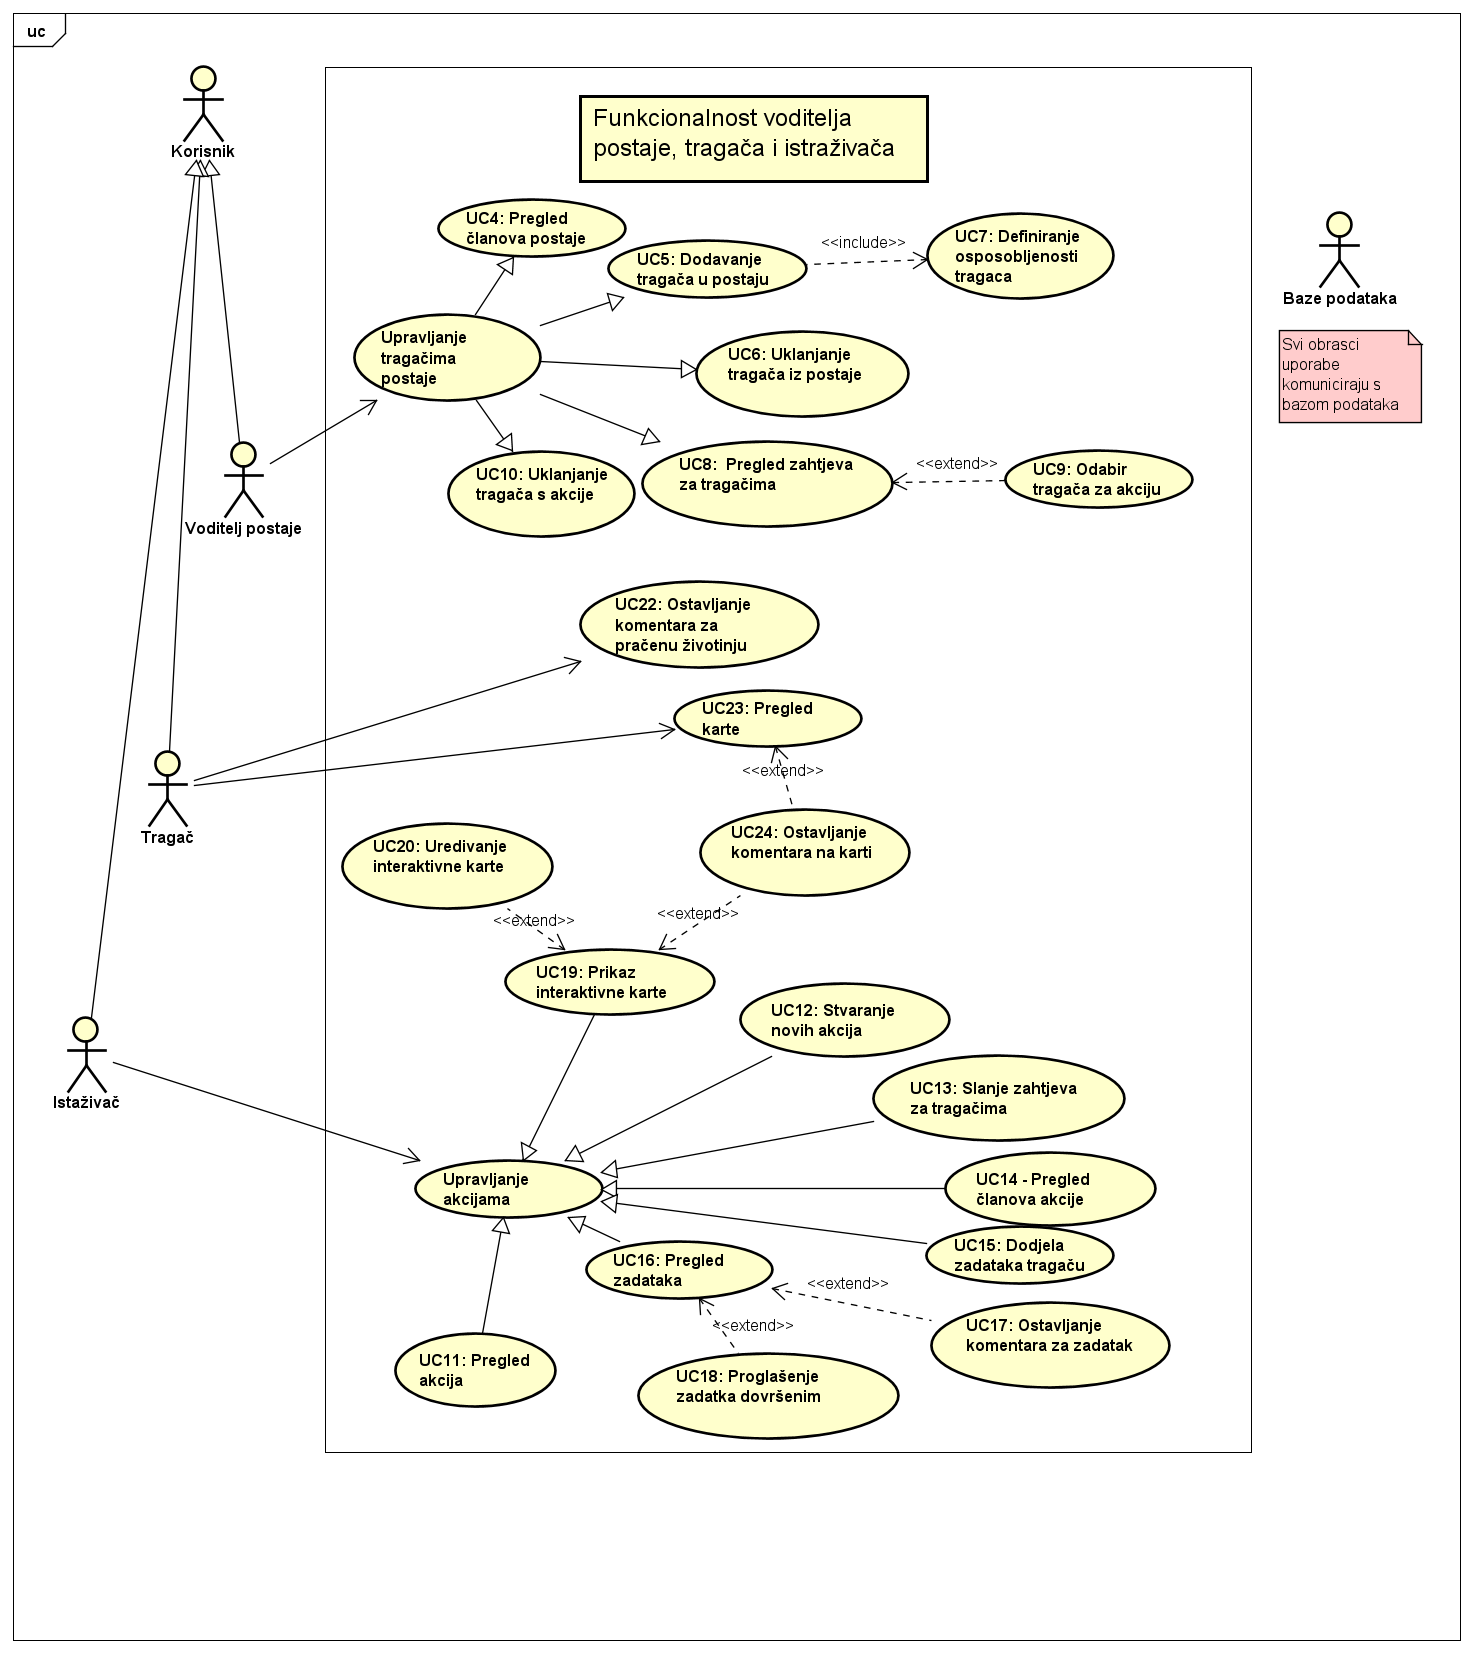
\includegraphics[scale=0.4]{dijagrami/voditelj-tragac-istrazivac-dijagram.PNG} 
						\centering
						\caption{Dijagram obrasca uporabe, voditelja postaje, tragača i istraživača}
						\label{fig:promjene}
					\end{figure}
					
			\eject				
				
			\subsection{Sekvencijski dijagrami}
			
				\subsubsection{Obrazac uporabe UC9 - Odabir tragača za akciju}
				Voditelj postaje šalje zahtjev za prikazom popisa pristiglih zahtjeva za alociranjem tragača za sudjelovanje u akciji. Poslužitelj dohvaća podatke o pristiglim zahtjevima i prikazuje ih. Voditelj odabire koji zahtjev želi detaljnije pregledati. Poslužitelj dohvaća pojedinosti o zahtjevu i prikazuje ih. Voditelj zatim šalje zahtjev za odabirom tragača koji će sudjelovati u akciji. Poslužitelj dohvaća tragače koji su raspoloživi. Raspoloživi tragači su oni koji u tom trenutku ne sudjeluju u niti jednoj akciji. U slučaju da takvih tragača ne postoji, poslužitelj ispisuje poruku "Nema raspoloživih tragača". U suprotnom, poslužitelj prikaže popis raspoloživih tragača.  Voditelj postaje zatim bira koje tragače želi dodati u akciju sve dok ne pošalje zahtjev za potvrdom odabira. Tada poslužitelj sprema odabir u bazu podataka.
				
				\eject
				
				\begin{figure}[H]
					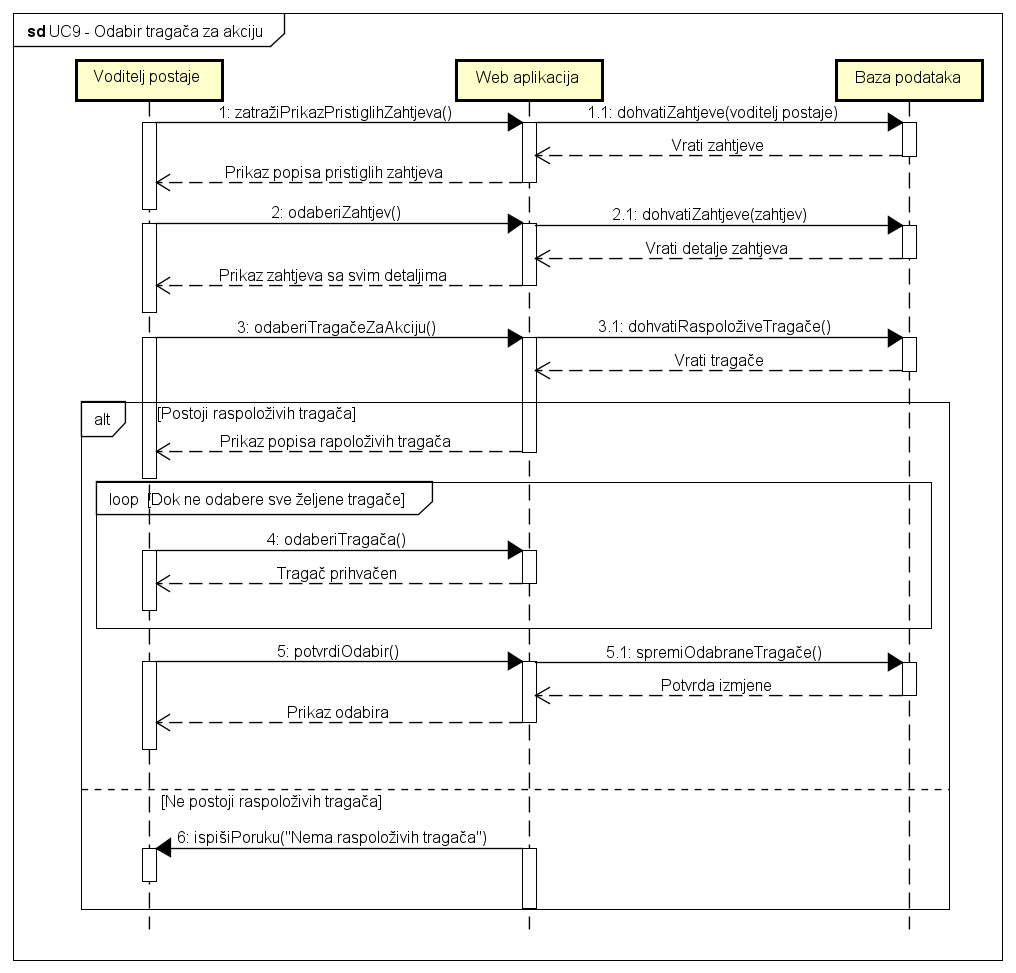
\includegraphics[scale=0.6]{dijagrami/UC9-Odabir tragača za akciju} 
					\centering
					\caption{Sekvencijski dijagram za UC9}
					\label{fig:promjene}
				\end{figure}
				
				\eject
				
				\subsubsection{Obrazac uporabe UC15 - Dodjela zadatka tragaču}
				Istraživač šalje zahtjev za prikazom akcija u kojima sudjeluje. Poslužitelj dohvaća podatke o istraživačevim akcijama i prikazuje ih. Istraživač odabire koju akciju želi detaljni pregledati. Poslužitelj dohvaća pojedinosti o akciji i prikazuje ih. Istraživač zatim šalje zahtjev za pregled tragača koji sudjeluju u akciji. Poslužitelj dohvaća tragače koji sudjeluju u akciji i prikazuje ih. Istraživač odabire tragača i poslužitelj bilježi taj odabir. Istraživač zatim šalje zahtjev o dodjeli zadatke odabranom tragaču. Poslužitelj dohvaća spremljenu kartu korištenu za ovu akciju i prikazuje ju zajedno s dijelom namijenjenim za odabir uređaja kojeg istraživač želi da se postavi(kamera ili uređaj za praćenje). Istraživač zatim na karti označava kojom rutom želi da se tragač kreće i do koje odredišne lokacije. Poslužitelj bilježi odabranu rutu. Istraživač onda bira između ponuđenih uređaja što poslužitelj također bilježi. Na kraju, istraživač potvrđuje dodjelu zadatka odabranom tragaču. Poslužitelj sprema u bazu podataka novi zadatak s svim navedenim specifikacijama i naznačuje tragača kojem je namijenjen. 
				
				\eject
				
				\begin{figure}[H]
					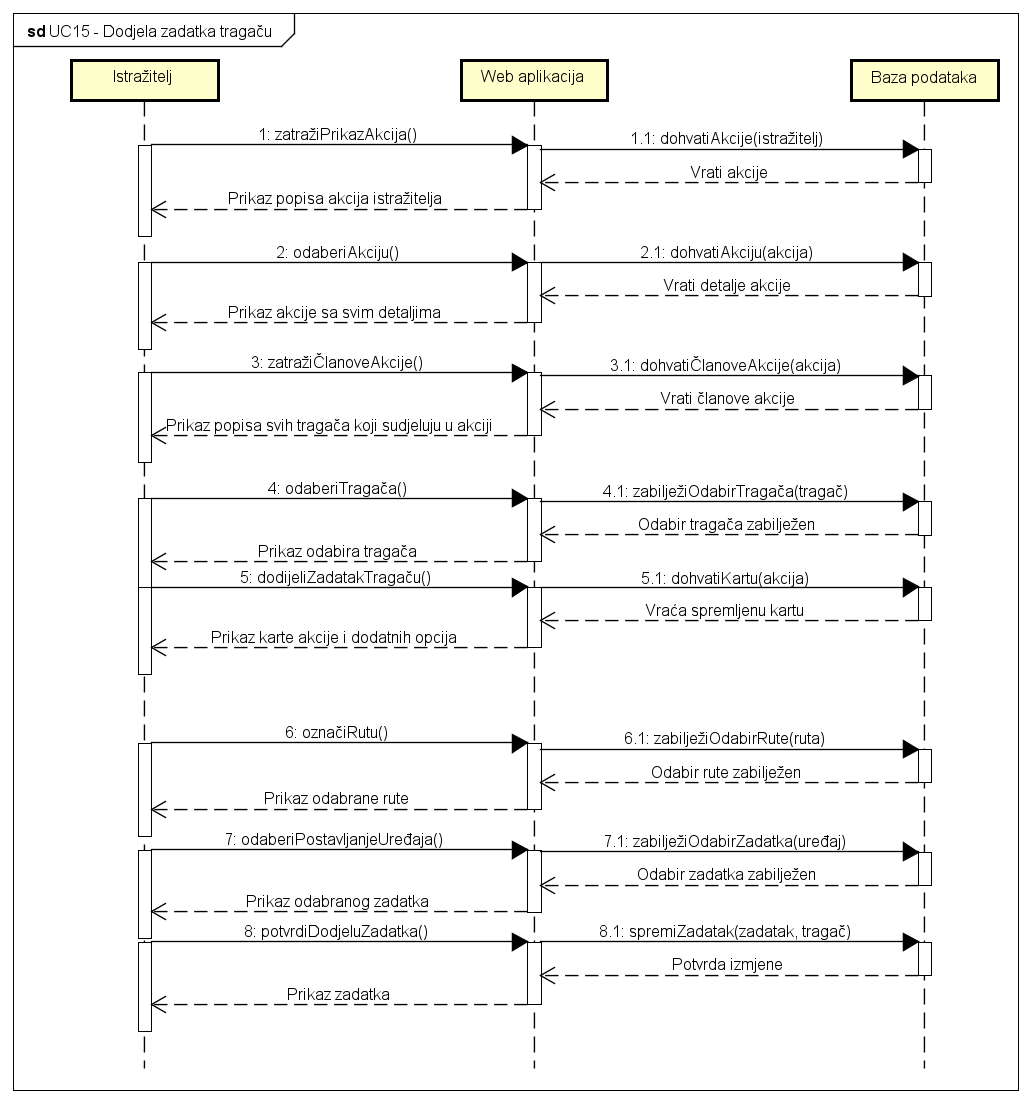
\includegraphics[scale=0.6]{dijagrami/UC15-Dodjela zadatka tragaču} 
					\centering
					\caption{Sekvencijski dijagram za UC15}
					\label{fig:promjene}
				\end{figure}
				
				\eject
				
				
				\subsubsection{Obrazac uporabe U20 - Uređivanje interaktivne karte}
				Istraživač šalje zahtjev za prikazom interaktivne karte. Poslužitelj dohvaća podatke o posljednjom spremljenom odabiru o prikazu informacija na karti i prikazuje ih. Istraživač zatim šalje zahtjev o uređivanju karte. Poslužitelj dohvaća podatke o svim mogućim informacijama koje mogu biti prikazane na karti i prikazuje ih istraživaču. Istraživač sada šalje zahtjev s odabirom koje informacije želi da budu prikazane. Poslužitelj provjerava je li odabrana opcija prikaza povijesnih pozicija svih praćenih životinja ili povijesnih pozicija svih tragača koji sudjeluju u akciji. Ako jest, onda poslužitelj prikazuje opcije filtriranja. U slučaju prikaza povijesnih pozicija svih praćenih životinja, podaci mogu biti filtrirani po vrsti ili pojedinačno po jedinki, dok prikaz povijesnih pozicija svih tragača koji sudjeluju u akciji može biti filtriran po tipu prijevoza ili pojedinačno po tragaču. Istraživač šalje zahtjev s odabirom kako želi da informacija bude filtrirana. Poslužitelj dohvaća informaciju s primijenjenim filtriranjem iz baze podataka, a u slučaju da je pri odabiru informacija bio odabran prikaz trenutnih pozicija praćenih životinja ili tragača, onda poslužitelj dohvaća tu informaciju bez ikakvog dodatnog filtriranja. Istraživač zatim šalje potvrdu za primjenu novog uređenja. Poslužitelj zatim sprema odabir u bazu podataka te prikazuje novonastalu kartu.
				\eject
				\begin{figure}[H]
					\includegraphics[scale=0.5]{dijagrami/UC20-Uređivanje interaktivne karte.PNG} 
					\centering
					\caption{Sekvencijski dijagram za UC20}
					\label{fig:promjene}
				\end{figure}
				
			\eject
		\section{Ostali zahtjevi}
		
			\begin{itemize}
				\item Web aplikaciju treba implementirati koristeći objektno-orijentirane jezike.
				\item Korisničko sučelje pri unosu i prikazu podataka treba podržavati hrvatski jezik uključujući dijakritičke znakove. 
				\item Potrebno je osigurati obranu sustava od pogrešnog korištenja korisničkog sučelja s dodatnim provjerama valjanosti.
				\item Sustav mora podržavati veći broj korisnika u stvarnom vremenu.
				\item Korisničko sučelje mora biti jednostavno i intuitivno za uporabu.
				\item Sustav je potrebno oblikovati na način koji pridonosi ponovnoj uporabi kao što je uvođenje kopči u program. 
				\item Programska potpora treba biti pripremljena za promjene u budućnosti. 
				\item Sustav mora odgovoriti na zahtjev korisnika u roku od nekoliko sekundi. 
				\item Pristup bazi podataka mora biti dobro zaštićen. 
				\item Dohvat sadržaja iz baze podataka trebao bi biti brz i učinkovit. 
				\item Programski proizvod treba raditi na što većem broju različitih platformi što se omogućuje korištenjem programskih jezika neovisnih o platformi.
				\item Komunikacija između web klijenta i web poslužitelja odvija se preko HTTPS protokola. 
			\end{itemize}
		 
			 
			 
			 
	
	\chapter{Arhitektura i dizajn sustava}
		
	Arhitektura se moze podijeliti na tri podsustava:
	
	\begin{itemize}
		\item Web posluzitelj
		\item Web aplikacija
		\item Baza podataka
	\end{itemize}

	
	\textit{Web preglednik} je alat koji omogućava korisnicima pregledavanje web stranica i njihovih povezanih multimedijalnih sadržaja. Svaki internetski preglednik djeluje kao prevoditelj, jer interpretira web stranice napisane u kodu kako bi ih prikazao korisnicima na razumljiv način. Korisnici putem web preglednika šalju zahtjeve web poslužitelju.
	
	\textit{Web poslužitelj} je ključni element u radu web aplikacije. Njegova glavna uloga je olakšavanje komunikacije između klijenta i aplikacije putem HTTP protokola. Poslužitelj pokreće web aplikaciju i prenosi joj zahtjev.
	
	\textit{Web aplikacija} služi korisniku za obradu željenih zahtjeva. Aplikacija obrađuje zahtjev, pristupa bazi podataka prema potrebi i putem poslužitelja vraća korisniku odgovor u obliku HTML dokumenta koji se prikazuje u web pregledniku.
	
	\textit{Baza podataka} ima svrhu pohranjivanja i upravljanja strukturiranim podacima koji se koriste u aplikaciji. Svaki put kad korisnik šalje zahtjev putem web preglednika, web aplikacija može pristupiti bazi podataka kako bi dohvatila ili ažurirala potrebne informacije. Baza podataka omogućava učinkovit pristup, pretraživanje i manipulaciju podacima, što je ključno za pravilan rad web aplikacije.
	
	Za izradu naše web aplikacije odabrali smo programski jezik Java zajedno s Springboot radnim okvirom, kao i programski jezik JavaScript. Razvojna okruženja koja koristimo su Visual Studio Code i IntelliJ. Arhitektura sustava temelji se na MVC (Model-View-Controller) konceptu, koji je podržan od strane Springboot radnog okvira i nudi gotove predloške koji olakšavaju razvoj web aplikacije. Kao poslužitelja baze podataka smo koristili PostgreSQL.
	
	MVC koncept donosi neovisnost u razvoju pojedinih dijelova aplikacije, što olakšava testiranje, kao i dodavanje novih svojstava u sustav. Sastoji se od:
	
	\begin{itemize}
		\item \textbf{Model} - Središnja komponenta sustava koja predstavlja dinamičke strukture podataka neovisne o korisničkom sučelju. Upravlja podacima, logikom i pravilima aplikacije, te prima ulazne podatke od Controllera.
		\item \textbf{View} - Ovdje se prikazuju podaci, primjerice u obliku grafova. Moguća su različita sučelja za prikaz informacija, poput grafičkog ili tabličnog prikaza podataka.
		\item \textbf{Controller} - Prima ulaze i prilagođava ih za daljnju interakciju s Modelom ili Viewom. Upravlja korisničkim zahtjevima i temeljem njih izvodi daljnje interakcije s ostalim elementima sustava.
	\end{itemize}
		

		

				
		\section{Baza podataka}
				
				Za bazu podataka koristi se relacijska baza podataka. Svaka tablica ima svoje ime i atribute. Vrste atributa koji se mogu nalaziti u tablici su primarni ključ, strani ključ ili atribut s nekom informacijom vezanom za tablicu. Baza podataka sastoji se od tablica:
		
				\begin{packed_item}
					\item AppUser
					\item ConfirmationToken
					\item StationManager
					\item SearcherInTheField
					\item Action
					\item Request
					\item Station
					\item Qualification
					\item Animal
					\item Location
				\end{packed_item}
				
				
		
			\subsection{Opis tablica}
			

				U tablici \textbf{AppUser} pohranjuju se podaci o svim korisnicima: \textit{id, userName, image, firstName, lastName, email, password, locked, enabled}. Primarni ključ je \textit{id}, i nema stranih ključeva. U njoj se nalaze svi korisnici, odnosno sve vrste korisnika. Korisnike dalje razlikujemo na tragače koji imaju svoje dodatne atribute u tablici \textbf{SearcherInTheField} i voditelje postaja koji imaju svoje dodatne atribute u tablici \textbf{StationManager}. Istraživači nemaju svoju posebnu tablicu jer je nepotrebna, nemaju svoje dodatne atribute koje moramo spremiti, a jedino za što su nam potrebni su akcije, a za to imamo id spremljen pod \textit{begun} u tablici \textbf{Action} pa tako dobijemo sve ostale podatke o istraživaču. S atributom \textit{id} je u odnosu One-to-One s tablicama \textbf{StationManager} i \textbf{SearcherInTheField} i u odnosu One-to-Many s tablicama \textbf{ConfirmationToken} i \textbf{Action}.

				
				
				\begin{longtblr}[
					label=none,
					entry=none
					]{
						width = \textwidth,
						colspec={|X[6,l]|X[6, l]|X[20, l]|}, 
						rowhead = 1,
					} %definicija širine tablice, širine stupaca, poravnanje i broja redaka naslova tablice
					\hline \SetCell[c=3]{c}{\textbf{AppUser}}	 \\ \hline[3pt]
					\SetCell{LightGreen}id & BIGINT	&  	id korisnika 	\\ \hline
					userName	& VARCHAR &  korisničko ime 	\\ \hline 
					image & BYTEA &  heksadekatski zapis korisničke slike  \\ \hline 
					firstName & VARCHAR	&  ime korisnika  \\ \hline 
					lastName & VARCHAR	&  prezime korisnika  \\ \hline 
					email & VARCHAR	&  email korisnika  \\ \hline 
					password & VARCHAR	&  lozinka korisnika  \\ \hline 
					locked & BOOLEAN & je li korisnika potvrdio admin \\ \hline
					enabled & BOOLEAN & je li korisnik potvrđen emailom \\ \hline
				\end{longtblr}
				
				U tablici \textbf{ConfirmationToken} pohranjuju se podaci za token za potvrdu poslanu korisniku: \textit{id, token, createdAt, expiresAt, confirmedAt, user}. Svaki token je povezan s korisnikom kojem je poslan preko \textit{user} u koji se sprema id korisnika. Primarni ključ je \textit{id}, a strani ključ je \textit{user}. S atributom \textit{user} je u odnosu Many-to-One s tablicom \textbf{AppUser}.
				
				\begin{longtblr}[
					label=none,
					entry=none
					]{
						width = \textwidth,
						colspec={|X[6,l]|X[6, l]|X[20, l]|}, 
						rowhead = 1,
					} %definicija širine tablice, širine stupaca, poravnanje i broja redaka naslova tablice
					\hline \SetCell[c=3]{c}{\textbf{ConfirmationToken}}	 \\ \hline[3pt]
					\SetCell{LightGreen}id & BIGINT	&  	id tokena 	\\ \hline
					token & VARCHAR & token \\ \hline
					createdAt & TIMESTAMP & vrijeme kada je token stvoren \\ \hline
					expiersAt & TIMESTAMP & vrijeme kada token ističe \\ \hline
					confirmedAt & TIMESTAMP & vrijeme kada je token potvrđen \\ \hline
					\SetCell{LightBlue}user	& BIGINT &  id korisnika kojemu je poslan token \\ \hline  
				\end{longtblr}

				U tablici \textbf{StationManager} pohranjuju se dodatni podaci za voditelja postaje: \textit{id, station}. U \textit{id} se sprema id korisnika koji je voditelj postaje, a u \textit{station} se sprema id postaje. Primarni ključ i ujedno i strani ključ je \textit{id} i također je strani ključ \textit{station}. S atributom \textit{id} je u odnosu One-to-One s tablicom \textbf{AppUser}, s atributom \textit{station} je u odnosu One-to-One s tablicom \textbf{Station}.

				
				\begin{longtblr}[
					label=none,
					entry=none
					]{
						width = \textwidth,
						colspec={|X[6,l]|X[6, l]|X[20, l]|}, 
						rowhead = 1,
					} %definicija širine tablice, širine stupaca, poravnanje i broja redaka naslova tablice

					\hline \SetCell[c=3]{c}{\textbf{StationManager}}	 \\ \hline[3pt]
					\SetCell{LightGreen}id & BIGINT	&  	id korisničkog računa voditelja 	\\ \hline
					\SetCell{LightBlue}station & BIGINT	&  	id postaje koju vodi voditelj 	\\ \hline
				\end{longtblr}
			

			U tablici \textbf{SearcherInTheField} pohranjuju se dodatni podaci za tragača: \textit{id, station, qualification}. U \textit{id} je spremljen id korisnika koji je tragač, u \textit{station} je pohranjen id postaje kojoj tragač pripada, a u \textit{qualification} je pohranjen id kvalifikacije koju tragač ima. Primarni ključ i ujedno i strani ključ je \textit{id} i također je strani ključ \textit{station} i \textit{qualification}. S atributom \textit{id} je u odnosu One-to-One s tablicom \textbf{AppUser}, s atributom \textit{station} je u odnosu Many-to-One s tablicom \textbf{Station}, s atributom \textit{qualification} je u odnosu Many-to-One s tablicom \textbf{Qualification}, s atributom \textit{id} je u odnosu One-to-Many s tablicom \textbf{Request} i  s atributom \textit{id} je u odnosu One-to-Many s tablicom \textbf{Location}.


			
				\begin{longtblr}[
					label=none,
					entry=none
					]{
						width = \textwidth,
						colspec={|X[10,l]|X[6, l]|X[20, l]|}, 
						rowhead = 1,
					} %definicija širine tablice, širine stupaca, poravnanje i broja redaka naslova tablice

					\hline \SetCell[c=3]{c}{\textbf{SearcherInTheField}}	 \\ \hline[3pt]
					\SetCell{LightGreen}id & BIGINT	&  	id korisničkog računa tragača 	\\ \hline
					\SetCell{LightBlue}station & BIGINT	&  	id postaje kojoj pripada 	\\ \hline
					\SetCell{LightBlue}qualification	& BIGINT &  id osposobljenosti tragača 	\\ \hline  
				\end{longtblr}
			

			U tablici \textbf{Action} pohranjuju se podaci o akciji: \textit{id, begun, description, comment}. U \textit{id} se sprema id akcije, u \textit{begun} se sprema id istraživača koji je pokrenuo akciju, odnosno id korisnika koji je pokrenuo akciju. \textit{Description} je opis akcije, odnosno što se radi i koji je cilj i \textit{comment} je dodatni komentar za akciju. Primarni ključ je \textit{id}, strani ključ je \textit{begun}. S atributom \textit{begun} je u odnosu Many-to-One s tablicom \textbf{AppUser} i s atributom \textit{id} je u odnosu One-to-Many s tablicom \textbf{Request}.


			
			\begin{longtblr}[
				label=none,
				entry=none
				]{
					width = \textwidth,
					colspec={|X[6,l]|X[6, l]|X[20, l]|}, 
					rowhead = 1,
				} %definicija širine tablice, širine stupaca, poravnanje i broja redaka naslova tablice
				
				\hline \SetCell[c=3]{c}{\textbf{Action}}	 \\ \hline[3pt]
				\SetCell{LightGreen}id & BIGINT	&  	id akcije 	\\ \hline
				\SetCell{LightBlue}begun & BIGINT	&  	id korisnika (istraživača) koji je započeo akciju 	\\ \hline
				description	& TEXT &  opis akcije 	\\ \hline
				comment & TEXT &  komentar za akciju 	\\ \hline  
			\end{longtblr}
			

			U tablici \textbf{Request} pohranjuju se podaci za zahtjev za tragačem: \textit{id, action, searcher, description, qualification, completed}. U \textit{id} je spremljen id zahtjeva, u \textit{action} je spremljen id akcije kojoj taj zahtjev pripada, odnosno zahtjevi se odnose na pojedini posao koji treba napraviti u pojedinoj akciji pa se u \textit{action} sprema id akcije kojoj taj posao pripada, \textit{description} služi kao opis posla koji tragač treba napraviti, u \textit{searcher} se sprema id tragača kojemu je dodijeljen posao, \textit{qualification} je id kvalifikacije potrebne za obavljanje posla i u \textit{completed} se sprema je li tragač izvršio taj posao ili nije. Primarni ključ je \textit{id}, strani ključevi su \textit{action}, \textit{searcher} i \textit{qualification}. S atributom \textit{action} je u odnosu Many-to-One s tablicom \textbf{Action}, s atributom \textit{searcher} je u odnosu Many-to-One s tablicom \textbf{SearcherInTheField} i s atributom \textit{qualification} je u odnosu One-to-One s tablicom \textbf{Qualification}.


			
			\begin{longtblr}[
				label=none,
				entry=none
				]{
					width = \textwidth,
					colspec={|X[6,l]|X[6, l]|X[20, l]|}, 
					rowhead = 1,
				} %definicija širine tablice, širine stupaca, poravnanje i broja redaka naslova tablice

				\hline \SetCell[c=3]{c}{\textbf{Request}}	 \\ \hline[3pt]
				\SetCell{LightGreen}id & BIGINT	&  	id zahtjeva 	\\ \hline
				\SetCell{LightBlue}action & BIGINT	&  	id akcije kojoj pripada zahtjev 	\\ \hline
				\SetCell{LightBlue}searcher & BIGINT	&  	id tragača koji je dobio zahtjev 	\\ \hline
				description	& TEXT &  opis  što tragač mora napraviti 	\\ \hline 
				\SetCell{LightBlue} qualification & TEXT & potrebne kvalifikacije \\ \hline
				completed & BOOLEAN & je li zahtjev završen ili ne \\ \hline
			\end{longtblr}
			

			U tablici \textbf{Station} pohranjuju se podaci za postaju: \textit{id, name}. U \textit{id} je spremljen id postaje, a u \textit{name} je spremljeno ime postaje. Primarni ključ je \textit{id} i nema stranih ključeva. S atributom \textit{id} je u odnosu One-to-One s tablicom \textbf{StationManager}, s atributom \textit{id} je u odnosu One-to-Many s tablicom \textbf{SearcherInTheField} i s atributom \textit{id} je u odnosu One-to-One s tablicom \textbf{Location}.


			
			\begin{longtblr}[
				label=none,
				entry=none
				]{
					width = \textwidth,
					colspec={|X[6,l]|X[6, l]|X[20, l]|}, 
					rowhead = 1,
				} %definicija širine tablice, širine stupaca, poravnanje i broja redaka naslova tablice

				\hline \SetCell[c=3]{c}{\textbf{Station}}	 \\ \hline[3pt]
				\SetCell{LightGreen}id & BIGINT	&  	id postaje 	\\ \hline
				name & VARCHAR & ime postaje \\ \hline
			\end{longtblr}

			U tablici \textbf{Qualification} pohranjuju se podaci za kvalifikacije: \textit{id, description, coverage, visibility}. U \textit{id} pohranjuje se id od kvalifikacije, u \textit{description} pohranjuje se opis kvalifikacije, u \textit{coverage} pohranjuje se područje pokriveno u kilometrima, za helikopter bi bilo npr. 10.00 km, u \textit{visibility} se sprema ocjena vidljivosti koja je obrnuto proporcionalna pokrivenosti, npr. helikopter ima veliku pokrivenost, ali se teško vide tragovi životinja pa ima manju vidljivost, dok hodanje šumom ima malu pokrivenost, ali se dobro vide tragovi koje ostave životinjei pa ima veliku vidljivost. Primarni ključ je \textit{id} i nema stranih ključeva. S atributom \textit{id} je u odnosu One-to-Many s tablicom \textbf{SearcherInTheField} i u odnosu One-to-One s tablicom \textbf{Request}.


			
			\begin{longtblr}[
				label=none,
				entry=none
				]{
					width = \textwidth,
					colspec={|X[10,l]|X[6, l]|X[20, l]|}, 
					rowhead = 1,
				} %definicija širine tablice, širine stupaca, poravnanje i broja redaka naslova tablice

				\hline \SetCell[c=3]{c}{\textbf{Qualification}}	 \\ \hline[3pt]
				\SetCell{LightGreen}id & BIGINT	&  	id osposobljenost 	\\ \hline
				description & VARCHAR & opis osposobljenosti (npr. pješice, autom,...) \\ \hline
				coverage & DOUBLE PRECISION & područje pokriveno u kilometrima \\ \hline
				visibility & BIGINT & ocjena vidljivosti na skali od 1 do 10 (1 je najgore, a 10 najbolje) \\ \hline
			\end{longtblr}
			

			U tablici \textbf{Animal} pohranjuju se podaci o životinji: \textit{id, species, comment}. U \textit{id} se pohranjuje id od životinje, u \textit{species} se pohranjuje vrsta životinje i u \textit{comment} se pohranjuje komentar o životinji, komentar može biti bilo što: izgled, ponašanje, zdravstveno stanje, ime životinje ili nešto drugo. Primarni ključ je \textit{id} i nema stranih ključeva. S atributom \textit{id} je u odnosu One-to-Many s tablicom \textbf{Location}.


			
			\begin{longtblr}[
				label=none,
				entry=none
				]{
					width = \textwidth,
					colspec={|X[6,l]|X[6, l]|X[20, l]|}, 
					rowhead = 1,
				} %definicija širine tablice, širine stupaca, poravnanje i broja redaka naslova tablice

				\hline \SetCell[c=3]{c}{\textbf{Animal}}	 \\ \hline[3pt]
				\SetCell{LightGreen}id & BIGINT	&  	id životinje 	\\ \hline
				species & VARCHAR & vrsta životinje \\ \hline
				comment & TEXT & komentar za životinju \\ \hline
			\end{longtblr}
			

			U tablici \textbf{Location} pohranjuju se podaci o lokaciji koja ima neku važnost: \textit{id, object, longitude, latitude, time, comment}. U \textit{id} se pohranjuje id lokacije, u \textit{object} se pohranjuje id objekta na nekoj lokaciji, objekt može biti tragač, životinja ili postaja. U \textit{longitude} i \textit{latitude} se spremaju geografska dužina i širina, u \textit{time} se sprema vrijeme kada je lokacija unesena i u \textit{comment} se sprema komentar za pojedinu lokaciju. Primarni ključ je \textit{id}, a strani ključ je \textit{object}. S atributom \textit{object} je u odnosu One-to-One s tablicom \textbf{Station}, Many-to-One s tablicom \textbf{Animal} i Many-to-One s tablicom \textbf{SearcherInTheField}.


			
			\begin{longtblr}[
				label=none,
				entry=none
				]{
					width = \textwidth,
					colspec={|X[6,l]|X[6, l]|X[20, l]|}, 
					rowhead = 1,
				} %definicija širine tablice, širine stupaca, poravnanje i broja redaka naslova tablice

				\hline \SetCell[c=3]{c}{\textbf{Location}}	 \\ \hline[3pt]
				\SetCell{LightGreen}id & BIGINT & id lokacije \\ \hline
				\SetCell{LightBlue}object & BIGINT	&  	id objekta na određenoj lokaciji 	\\ \hline
				longitude & DOUBLE PRECISION & geografska dužina \\ \hline
				latitude & DOUBLE PRECISION & geografska širina \\ \hline
				time & TIMESTAMP & vrijeme kada je lokacija spremljena \\ \hline
				comment & TEXT & komentar za lokaciju \\ \hline

			\end{longtblr}
			
			\subsection{Dijagram baze podataka}
				\begin{figure}[H]
					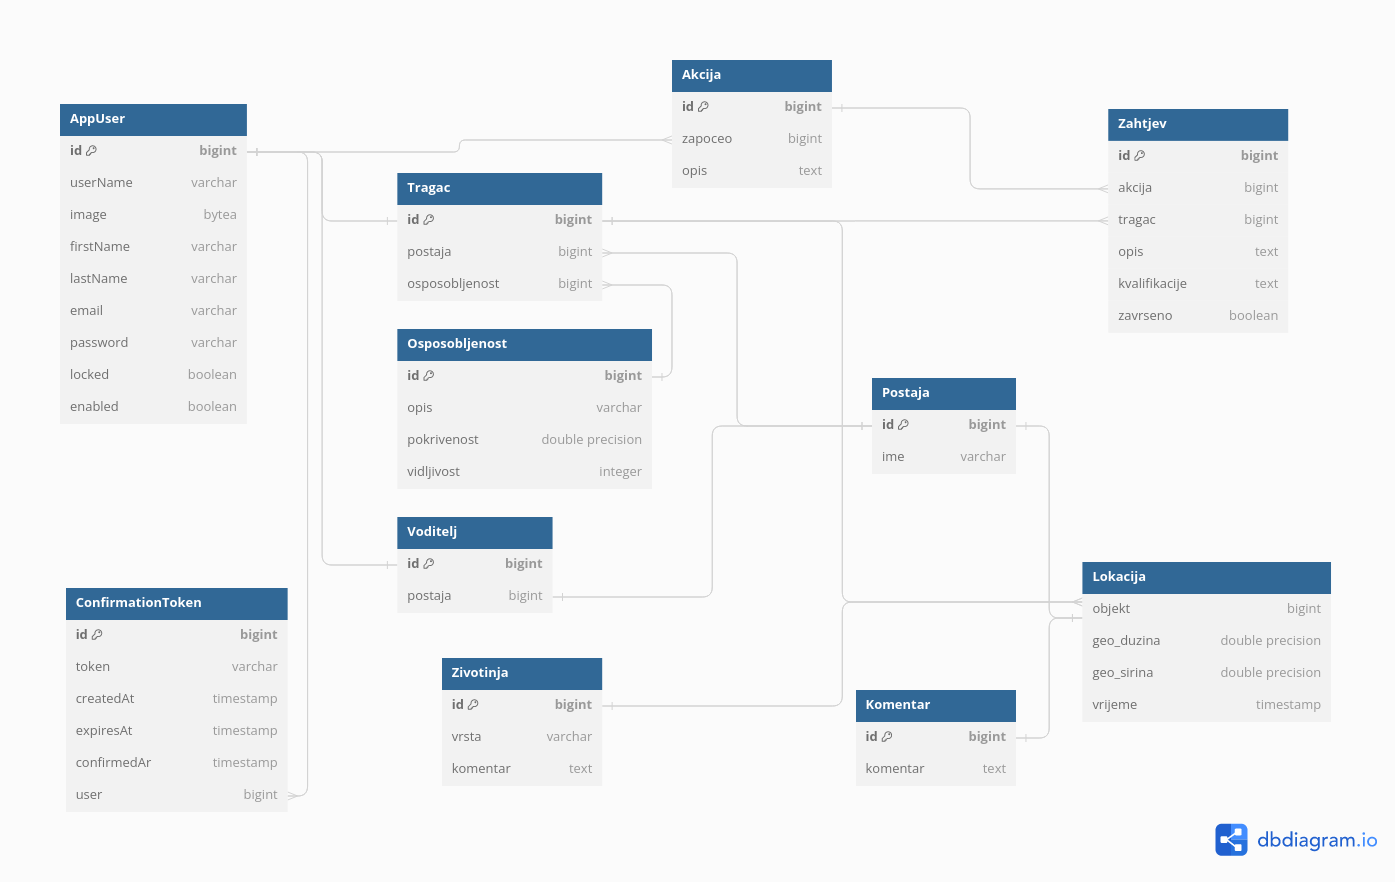
\includegraphics[scale=0.35]{dijagrami/dijagram_baze_podataka.png}
					\centering
					\caption{Dijagram baze podataka}
					\label{fig:promjene}
				\end{figure}
			\eject
			
			
		\section{Dijagram razreda}
		Dijagram razreda podijeljen je zbog bolje preglednosti na tri dijela: Controllers, Models i DTO. Prikazane su veze koje ostvaruju razredi unutar istog dijela dijagrama, a odnosi između razreda u različitim dijelovima mogu se zaključiti iz tipova atributa. Metode korištene u Controller razredima vraćaju \textit{ResponseEntity}, koji predstavlja HTTP odgovor, ili samo kod odgovora HTTP-a. U svom radu koriste objekte za prijenos podataka (DTO) i ostvaruju komunikaciju s klijentskom stranom.
			
			\begin{figure}[H]
				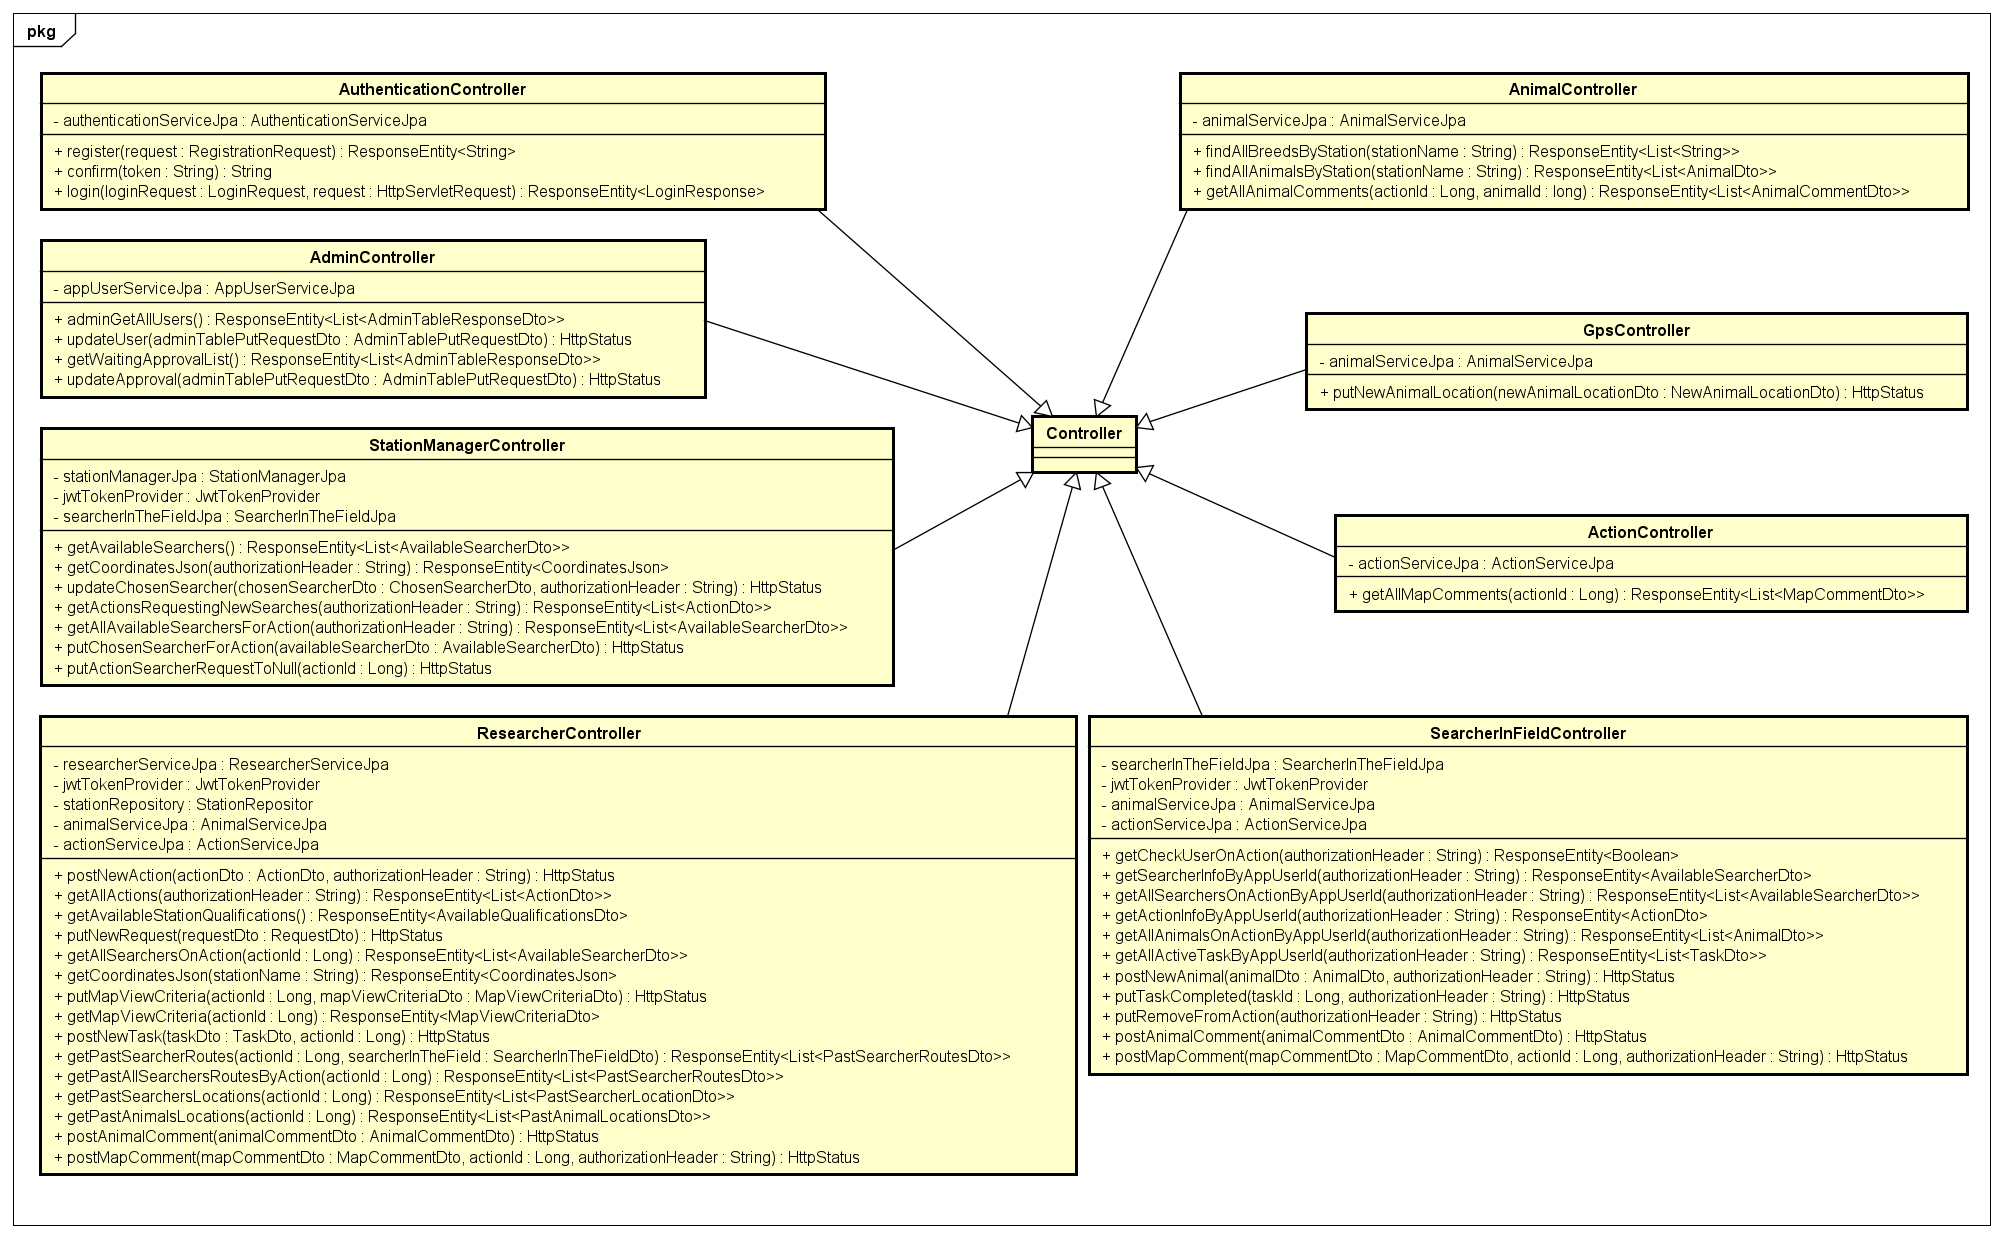
\includegraphics[scale=0.5]{dijagrami/Controllers.png} 
				\centering
				\caption{Dijagram razreda - dio Controllers}
				\label{fig:promjene}
			\end{figure}
			
			\begin{figure}[H]
				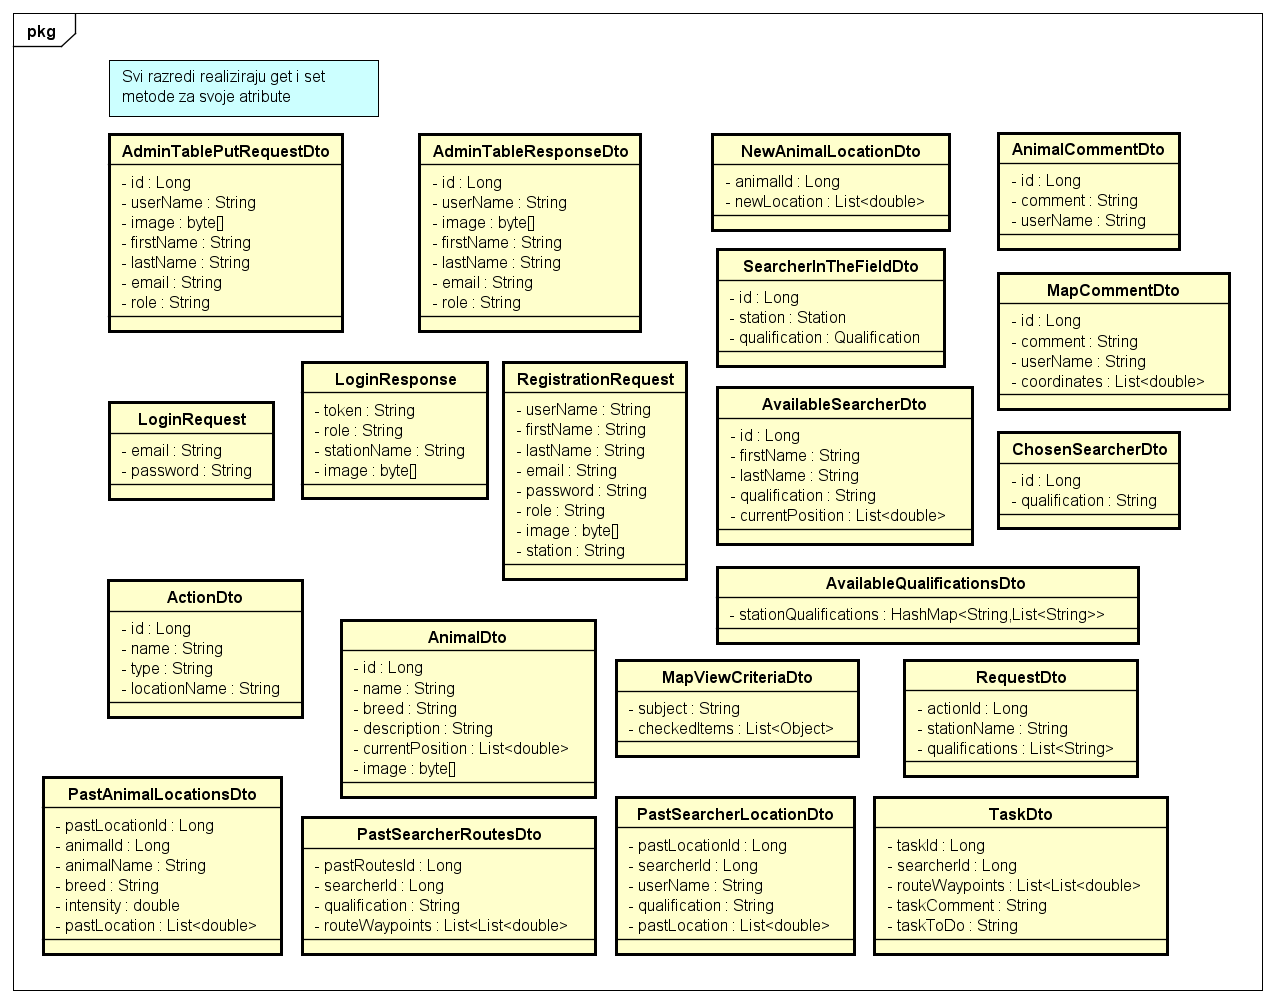
\includegraphics[scale=0.5]{dijagrami/DTO.png} 
				\centering
				\caption{Dijagram razreda - dio DTO}
				\label{fig:promjene}
			\end{figure}
			
			\begin{figure}[H]
				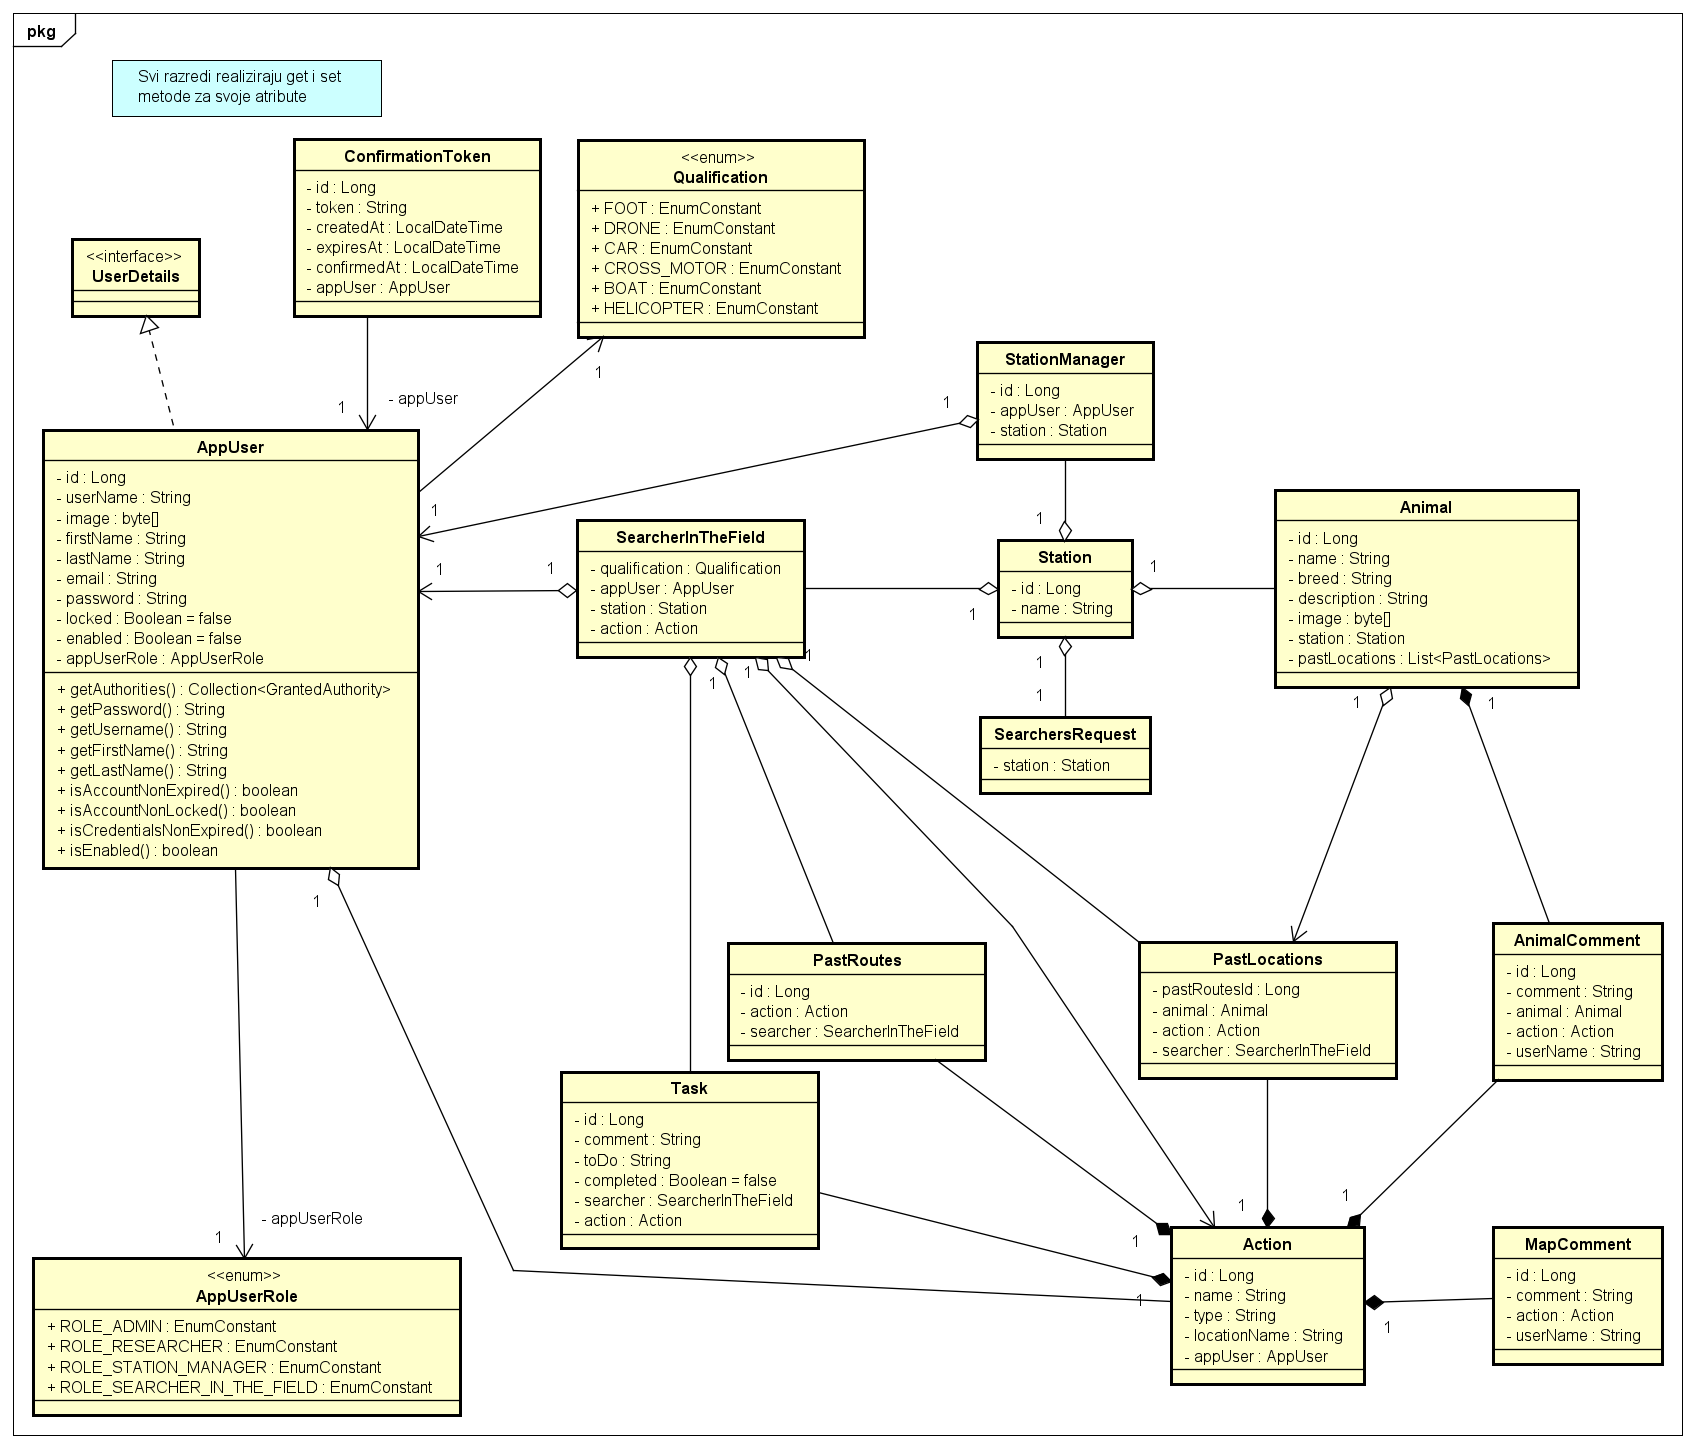
\includegraphics[scale=0.4]{dijagrami/Model.png} 
				\centering
				\caption{Dijagram razreda - dio Models}
				\label{fig:promjene}
			\end{figure}
			
			
			\eject
		
		\section{Dijagram stanja}
			
			
			Dijagrami stanja prikazuju kako sustav prelazi iz jednog stanja u drugo kao odgovor na događaje. Prijavljenom korisniku, u ovom slučaju istraživaču, prikazuje se početna stranica s nekoliko opcija: pregled vlastitih akcija, stvaranje nove akcije i pregled osobnih podataka. Nakon odabira opcije stvaranja nove akcije, korisniku se nudi mogućnost slanja zahtjeva za tragačima za pripadajuću akciju. U slučaju da nema slobodnih tragača, sustav obavijesti korisnika i čeka na idući zahtjev. Ako se istraživaču dodijele tragači, može im dodijeliti zadatke. Zatim ima opciju unosa komentara na zadatak. Odabirom opcije ,,Moje akcije“ , istraživač može vidjeti sve svoje akcije i pregledati njihove članove te završiti neku od akcija.  Također, istraživač može odabrati prikaz karte i urediti je po želji. Nakon toga može ostaviti komentar na karti.
			
			\begin{figure}[H]
				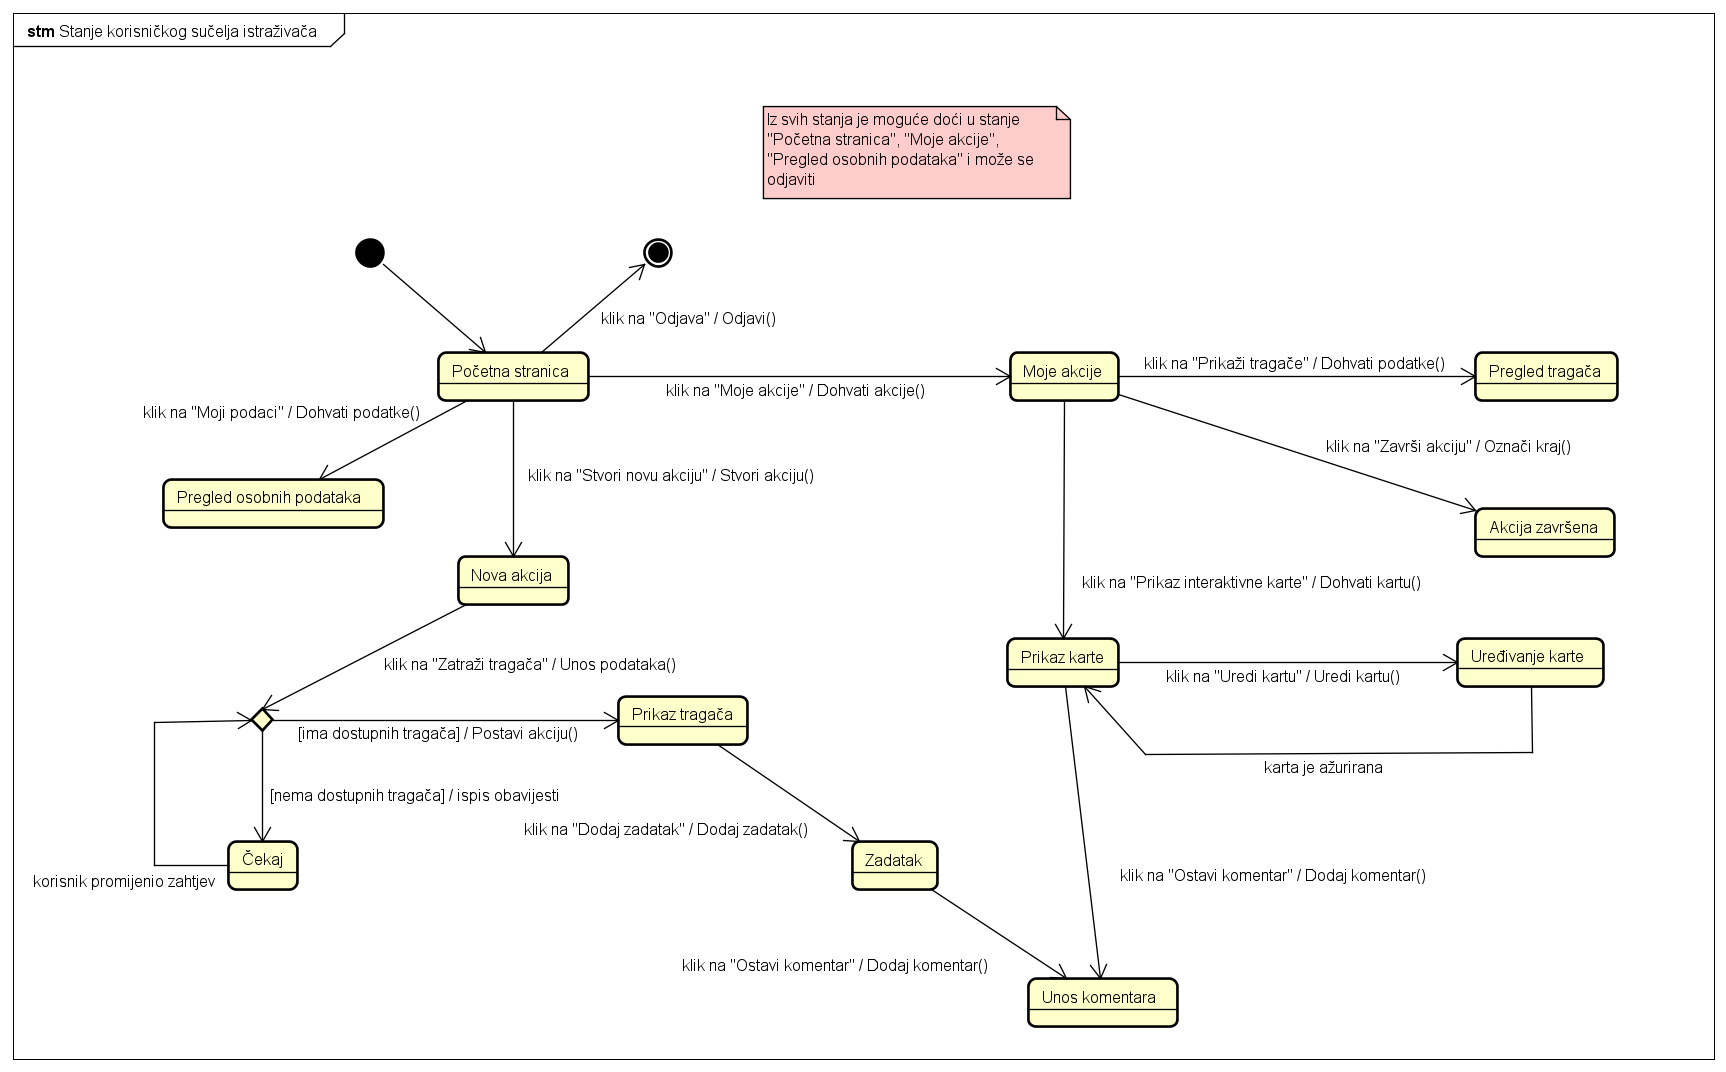
\includegraphics[scale=0.3]{dijagrami/DijagramStanja.png} 
				\centering
				\caption{Dijagram stanja}
				\label{fig:promjene}
			\end{figure}
			
			
			\eject 
		
		\section{Dijagram aktivnosti}
			
			Dijagrami aktivnosti upotrebljavaju se za modeliranje dinamičkog ponašanja sustava. Izvođenje aktivnosti prikazano je kroz niz akcija koje čine upravljačke tokove i tokove objekata. Prikazan je proces stvaranja nove akcije. Aktivnost započinje prijavom istraživača u sustav. Nakon uspješne prijave, istraživaču se prikazuje početna stranica. Odabirom opcije za stvaranje nove akcije aplikacija prikazuje formu za unos podataka o akciji. Istraživač unosi podatke o akciji, a sustav ih pohranjuje u bazu podataka. Zatim istraživač šalje zahtjev za tragačima, a aplikacija prikazuje formu za unos detalja o zahtjevu. Aplikacija prosljeđuje zahtjev voditelju postaje koji dodjeljuje tragače akciji (pretpostavlja se da ima dostupnih tragača). Popis tragača se pohranjuje u bazu i prikazuje u aplikaciji. Na zahtjev za dodjeljivanje zadatka nekom od tragača prikazuje se forma za unos zadatka. Zadatak se sprema u bazu podataka, a istraživač može unijeti i komentar o zadatku. Nakon završetka unosa svih podataka o akciji aplikacija prikazuje poruku da su svi podaci spremljeni i aktivnost završava.
			
			\begin{figure}[H]
				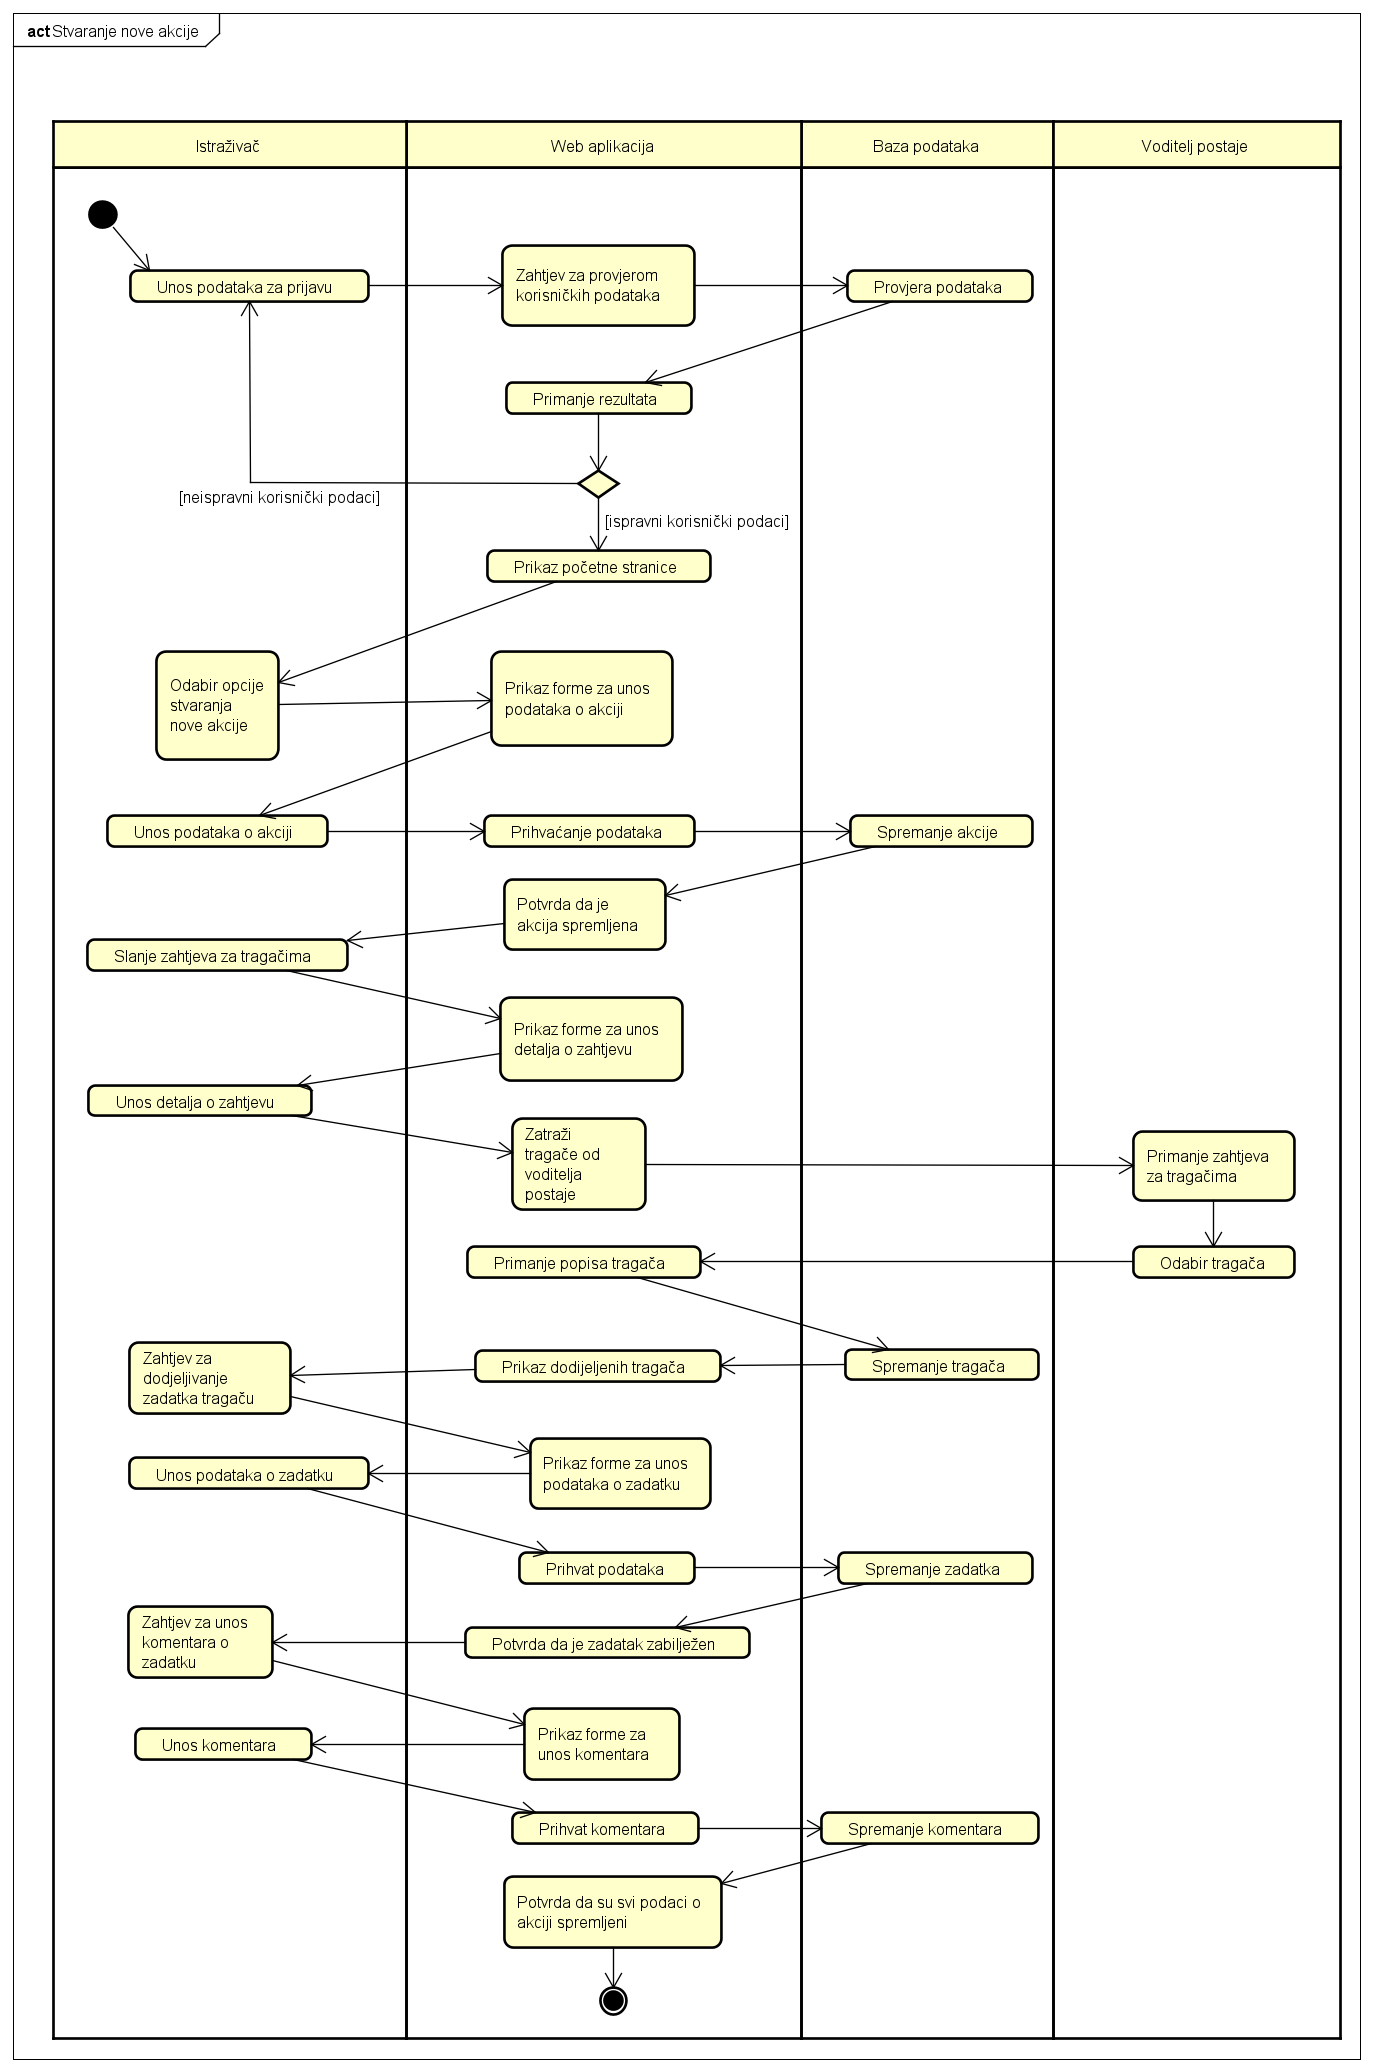
\includegraphics[scale=0.4]{dijagrami/DijagramAkt.png} 
				\centering
				\caption{Dijagram aktivnosti}
				\label{fig:promjene}
			\end{figure}
			
			\eject
		\section{Dijagram komponenti}
		
			\textbf{\textit{dio 2. revizije}}\\
		
			 \textit{Potrebno je priložiti dijagram komponenti s pripadajućim opisom. Dijagram komponenti treba prikazivati strukturu cijele aplikacije.}
	\chapter{Implementacija i korisničko sučelje}
		
		
		\section{Korištene tehnologije i alati}
		
			Tim je koristio \underline{WhatsApp}.\footnote[1]{https://www.whatsapp.com/} i \underline{Notion}.\footnote[2]{https://www.notion.so/} za komunikaciju unutar tima. Za izradu UML dijagrama korišten je \underline{Astah Professional}.\footnote[3]{https://astah.net/products/astah-professional/}, dok je za upravljanje izvornim kodom odabran \underline{Git}.\footnote[4]{https://git-scm.com/}. Udaljeni repozitorij projekta dostupan je na web platformi \underline{GitHub}.\footnote[5]{https://github.com/}.
			
			Kao razvojna okruženja korišteni su \underline{Visual Studio Code}.\footnote[6]{https://code.visualstudio.com/} i \underline{IntelliJ IDEA}.\footnote[7]{https://www.jetbrains.com/idea/}. Visual Studio Code je jednostavan uređivač koda s podrškom za razvojne operacije poput debugiranja, pokretanja zadataka i kontrolu verzija od tvrtke Microsoft, dok je IntelliJ popularno razvojno okruženje (IDE) razvijeno od strane tvrtke JetBrains. Namijenjeno je prvenstveno za rad s Java programskim jezikom.
			
			Aplikacija je napisana koristeći radni okvir \underline{Spring Boot}.\footnote[8]{https://spring.io/projects/spring-boot/} i jezik \underline{Java}.\footnote[9]{https://www.java.com/en/} za izradu backenda te \underline{React}.\footnote[10]{https://react.dev/} i jezik \underline{JavaScript}.\footnote[11]{https://www.javascript.com/} za izradu frontenda. React je besplatna i open-source JavaScript biblioteka za izgradnju korisničkih sučelja temeljenih na komponentama. Održava je Meta i zajednica pojedinačnih razvijatelja te tvrtki. Radni okvir Spring Boot je otvoreni, mikroservisni Java web okvir koji nudi Spring. Razvijen je kako bi pojednostavio proces izrade, konfiguracije i razmještanja Java aplikacija. 
			
			Baza podataka se nalazi na posluzitelju u oblaku \underline{Render}.\footnote[12]{https://render.com/}.
			
			
			\eject 
		
	
		\section{Ispitivanje programskog rješenja}
			
			\textbf{\textit{dio 2. revizije}}\\
			
			 \textit{U ovom poglavlju je potrebno opisati provedbu ispitivanja implementiranih funkcionalnosti na razini komponenti i na razini cijelog sustava s prikazom odabranih ispitnih slučajeva. Studenti trebaju ispitati temeljnu funkcionalnost i rubne uvjete.}
	
			
			\subsection{Ispitivanje komponenti}
			\textit{Potrebno je provesti ispitivanje jedinica (engl. unit testing) nad razredima koji implementiraju temeljne funkcionalnosti. Razraditi \textbf{minimalno 6 ispitnih slučajeva} u kojima će se ispitati redovni slučajevi, rubni uvjeti te izazivanje pogreške (engl. exception throwing). Poželjno je stvoriti i ispitni slučaj koji koristi funkcionalnosti koje nisu implementirane. Potrebno je priložiti izvorni kôd svih ispitnih slučajeva te prikaz rezultata izvođenja ispita u razvojnom okruženju (prolaz/pad ispita). }
			
			
			
			\subsection{Ispitivanje sustava}
			
			 \textit{Potrebno je provesti i opisati ispitivanje sustava koristeći radni okvir Selenium\footnote{\url{https://www.seleniumhq.org/}}. Razraditi \textbf{minimalno 4 ispitna slučaja} u kojima će se ispitati redovni slučajevi, rubni uvjeti te poziv funkcionalnosti koja nije implementirana/izaziva pogrešku kako bi se vidjelo na koji način sustav reagira kada nešto nije u potpunosti ostvareno. Ispitni slučaj se treba sastojati od ulaza (npr. korisničko ime i lozinka), očekivanog izlaza ili rezultata, koraka ispitivanja i dobivenog izlaza ili rezultata.\\ }
			 
			 \textit{Izradu ispitnih slučajeva pomoću radnog okvira Selenium moguće je provesti pomoću jednog od sljedeća dva alata:}
			 \begin{itemize}
			 	\item \textit{dodatak za preglednik \textbf{Selenium IDE} - snimanje korisnikovih akcija radi automatskog ponavljanja ispita	}
			 	\item \textit{\textbf{Selenium WebDriver} - podrška za pisanje ispita u jezicima Java, C\#, PHP koristeći posebno programsko sučelje.}
			 \end{itemize}
		 	\textit{Detalji o korištenju alata Selenium bit će prikazani na posebnom predavanju tijekom semestra.}
			
			\eject 
		
		
		\section{Dijagram razmještaja}
			
			\textbf{\textit{dio 2. revizije}}
			
			 \textit{Potrebno je umetnuti \textbf{specifikacijski} dijagram razmještaja i opisati ga. Moguće je umjesto specifikacijskog dijagrama razmještaja umetnuti dijagram razmještaja instanci, pod uvjetom da taj dijagram bolje opisuje neki važniji dio sustava.}
			
			\eject 
		
		\section{Upute za puštanje u pogon}
		
			\textbf{\textit{dio 2. revizije}}\\
		
			 \textit{U ovom poglavlju potrebno je dati upute za puštanje u pogon (engl. deployment) ostvarene aplikacije. Na primjer, za web aplikacije, opisati postupak kojim se od izvornog kôda dolazi do potpuno postavljene baze podataka i poslužitelja koji odgovara na upite korisnika. Za mobilnu aplikaciju, postupak kojim se aplikacija izgradi, te postavi na neku od trgovina. Za stolnu (engl. desktop) aplikaciju, postupak kojim se aplikacija instalira na računalo. Ukoliko mobilne i stolne aplikacije komuniciraju s poslužiteljem i/ili bazom podataka, opisati i postupak njihovog postavljanja. Pri izradi uputa preporučuje se \textbf{naglasiti korake instalacije uporabom natuknica} te koristiti što je više moguće \textbf{slike ekrana} (engl. screenshots) kako bi upute bile jasne i jednostavne za slijediti.}
			
			
			 \textit{Dovršenu aplikaciju potrebno je pokrenuti na javno dostupnom poslužitelju. Studentima se preporuča korištenje neke od sljedećih besplatnih usluga: \href{https://aws.amazon.com/}{Amazon AWS}, \href{https://azure.microsoft.com/en-us/}{Microsoft Azure} ili \href{https://www.heroku.com/}{Heroku}. Mobilne aplikacije trebaju biti objavljene na F-Droid, Google Play ili Amazon App trgovini.}
			
			
			\eject 
	\chapter{Zaključak i budući rad}
		
		\textbf{\textit{dio 2. revizije}}\\
		
		 \textit{U ovom poglavlju potrebno je napisati osvrt na vrijeme izrade projektnog zadatka, koji su tehnički izazovi prepoznati, jesu li riješeni ili kako bi mogli biti riješeni, koja su znanja stečena pri izradi projekta, koja bi znanja bila posebno potrebna za brže i kvalitetnije ostvarenje projekta i koje bi bile perspektive za nastavak rada u projektnoj grupi.}
		
		 \textit{Potrebno je točno popisati funkcionalnosti koje nisu implementirane u ostvarenoj aplikaciji.}
		
		\eject 
	\chapter*{Popis literature}
		\addcontentsline{toc}{chapter}{Popis literature}
	 	
 		\textbf{\textit{Kontinuirano osvježavanje}}
	
		\textit{Popisati sve reference i literaturu koja je pomogla pri ostvarivanju projekta.}
		
		
		\begin{enumerate}
			
			
			\item  Programsko inženjerstvo, FER ZEMRIS, \url{http://www.fer.hr/predmet/proinz}
			
			
			\item  The Unified Modeling Language, \url{https://www.uml-diagrams.org/}
			
			\item  Astah Community, \url{http://astah.net/editions/uml-new}
			
			\item National Geographic https://www.nationalgeographic.com/culture/article/where-animals-go-tracking-maps
			
			\item USGC https://alaska.usgs.gov/products/data/tracking/tracking.php?groupid=4
			
			\item designmodo https://designmodo.com/create-css3-login-form/
			
			\item designmodo https://designmodo.com/create-css3-login-form/
			
			\item Volunteer Match https://www.volunteermatch.org/
			
			\item Movebank https://www.movebank.org/
			
			\item Wildme https://www.wildme.org/
			
			\item iNaturalist https://www.inaturalist.org/
			
			\item Wildbook for Iberian Lynx https://lynx.wildbook.org/
			
		\end{enumerate}
		
		 
	
	
	\begingroup
	\renewcommand*\listfigurename{Indeks slika i dijagrama}
	%\renewcommand*\listtablename{Indeks tablica}
	%\let\clearpage\relax
	\listoffigures
	%\vspace{10mm}
	%\listoftables
	\endgroup
	\addcontentsline{toc}{chapter}{Indeks slika i dijagrama}


	
	\eject 
		
	\chapter*{Dodatak: Prikaz aktivnosti grupe}
		\addcontentsline{toc}{chapter}{Dodatak: Prikaz aktivnosti grupe}
		
		\section*{Dnevnik sastajanja}
		
		\textbf{\textit{Kontinuirano osvježavanje}}\\
		
		 \textit{U ovom dijelu potrebno je redovito osvježavati dnevnik sastajanja prema predlošku.}
		
		\begin{packed_enum}
			\item  sastanak
			
			\item[] \begin{packed_item}
				\item Datum: u ovom formatu: \today
				\item Prisustvovali: I.Prezime, I.Prezime
				\item Teme sastanka:
				\begin{packed_item}
					\item  opis prve teme
					\item  opis druge teme
				\end{packed_item}
			\end{packed_item}
			
			\item  sastanak
			\item[] \begin{packed_item}
				\item Datum: u ovom formatu: \today
				\item Prisustvovali: I.Prezime, I.Prezime
				\item Teme sastanka:
				\begin{packed_item}
					\item  opis prve teme
					\item  opis druge teme
				\end{packed_item}
			\end{packed_item}
			
			%
			
		\end{packed_enum}
		
		\eject
		\section*{Tablica aktivnosti}
		
			\textbf{\textit{Kontinuirano osvježavanje}}\\
			
			 \textit{Napomena: Doprinose u aktivnostima treba navesti u satima po članovima grupe po aktivnosti.}

			\begin{longtblr}[
					label=none,
				]{
					vlines,hlines,
					width = \textwidth,
					colspec={X[7, l]X[1, c]X[1, c]X[1, c]X[1, c]X[1, c]X[1, c]X[1, c]}, 
					vline{1} = {1}{text=\clap{}},
					hline{1} = {1}{text=\clap{}},
					rowhead = 1,
				} 
			
				\SetCell[c=1]{c}{} & \SetCell[c=1]{c}{\rotatebox{90}{\textbf{Filip Ljubotina
				}}} & \SetCell[c=1]{c}{\rotatebox{90}{\textbf{Marko Pavić
			 }}} &	\SetCell[c=1]{c}{\rotatebox{90}{\textbf{Ana Vuksanović
		  }}} & \SetCell[c=1]{c}{\rotatebox{90}{\textbf{Lara Ćorić }}} &	\SetCell[c=1]{c}{\rotatebox{90}{\textbf{Katarina Klarić }}} & \SetCell[c=1]{c}{\rotatebox{90}{\textbf{Mihael Breznički-Herceg }}} &	\SetCell[c=1]{c}{\rotatebox{90}{\textbf{Noa Milin
	   }}} \\  
				Upravljanje projektom 		& 8 &  &  &  &  &  & \\ 
				Opis projektnog zadatka 	&  &  &  & 6 &  &  & \\ 
				
				Funkcionalni zahtjevi       &  & 2 &  &  &  &  &  \\ 
				Opis pojedinih obrazaca 	&  & 6 & 2 &  &  &  &  \\ 
				Dijagram obrazaca 			& 5 &  &  &  &  &  &  \\ 
				Sekvencijski dijagrami 		&  &  & 5 &  &  &  &  \\ 
				Opis ostalih zahtjeva 		&  &  &  &  & 1 &  &  \\ 

				Arhitektura i dizajn sustava	 &  & 1.5 &  &  &  &  &  \\ 
				Baza podataka				&  &  &  &  &  & 7 &   \\ 
				Dijagram razreda 			& 2 &  &  &  & 6 &  & 6  \\ 
				Dijagram stanja				&  &  &  &  &  &  &  \\ 
				Dijagram aktivnosti 		&  &  &  &  &  &  &  \\ 
				Dijagram komponenti			&  &  &  &  &  &  &  \\ 
				Korištene tehnologije i alati 		&  &  &  &  &  &  &  \\ 
				Ispitivanje programskog rješenja 	&  &  &  &  &  &  &  \\ 
				Dijagram razmještaja			&  &  &  &  &  &  &  \\ 
				Upute za puštanje u pogon 		&  &  &  &  &  &  &  \\  
				Dnevnik sastajanja 			&  &  &  &  &  &  &  \\ 
				Zaključak i budući rad 		&  &  &  &  &  &  &  \\  
				Popis literature 			&  &  &  &  &  &  &  \\  
				&  &  &  &  &  &  &  \\ \hline 
				\textit{izrada back end-a} 						& 20 &  &  &  &  &  &  \\  
				\textit{npr. izrada front end-a} 			& 5 &  & 15 &  &  &  &  \\ 
				\textit{deploy-anje aplikacije} 			& 5 &  &  &  &  &  &  \\
				 							&  &  &  &  &  &  &\\ 
			\end{longtblr}
					
					
		\eject
		\section*{Dijagrami pregleda promjena}
		
		\textbf{\textit{dio 2. revizije}}\\
		
		\textit{Prenijeti dijagram pregleda promjena nad datotekama projekta. Potrebno je na kraju projekta generirane grafove s gitlaba prenijeti u ovo poglavlje dokumentacije. Dijagrami za vlastiti projekt se mogu preuzeti s gitlab.com stranice, u izborniku Repository, pritiskom na stavku Contributors.}
		
	


\end{document} %naredbe i tekst nakon ove naredbe ne ulaze u izgrađen dokument 


